\documentclass{llncs}
%%%%%%%%%%%%%%%%%%%%%%
%%%%   PACKAGES   %%%%
%%%%%%%%%%%%%%%%%%%%%%
\usepackage{makeidx}
\usepackage{amsmath}
\usepackage{amssymb}
\usepackage{stmaryrd}
\usepackage{graphicx}
\usepackage{subfigure}
\usepackage{latexsym}
\usepackage{url}
\usepackage{color}
\usepackage{isabelle}
\usepackage{isabellesym}
\usepackage{theorem}

%%%%%%%%%%%%%%%%%%%%%%%%%%%%
%For Isabelle code
\newlength{\fminilength}
\newsavebox{\fminibox}
\newenvironment{fmini}[1][\linewidth]
  {\setlength{\fminilength}{#1\fboxsep-2\fboxrule}%
   \vspace{2ex}\noindent\begin{lrbox}{\fminibox}\begin{minipage}{\fminilength}%
   \mbox{ }\hfill\vspace{-2.5ex}}%
  {\end{minipage}\end{lrbox}\vspace{1ex}\hspace{0ex}%
   \framebox{\usebox{\fminibox}}}

\newenvironment{specification}
{\noindent\scriptsize
\tt\begin{fmini}\begin{tabbing}X\=X12345\=XXXX\=XXXX\=XXXX\=XXXX\=XXXX
\=\+\kill} {\end{tabbing}\normalfont\end{fmini}}
\def \twoSpaces {\ \ }
\def \oneSpace {\ }
\def \eqc {=_C }
\def \andc {\wedge_C }
\def \negc {\neg_C }
\def \orc {\vee_C }
\def \alt {$/\backslash$ }
\def \cat {:}
\def \dbRight {$\backslash\backslash$}
\def \iInv {iInv}
\def \iR {iR}
%%%%%%%%%%%%%%%%%%%%%%%%%%%%

%%%%%%%%%%%%%%%%%%%%%%%%%%%%
%for comments
\newcommand\JP[1]{\textcolor{magenta}{JP: #1}}
\newcommand\lyj[1]{\textcolor{green}{lyj: #1}}
%%%%%%%%%%%%%%%%%%%%%%%%%%%

%%%%%%%%%%%%%%%%%%%%%%%%%%%
% Additional math operators
%%%%%%%%%%%%%%%%%%%%%%%%%%%

\usepackage[colorlinks,
            linkcolor=black,
            anchorcolor=black,
            citecolor=blue,
            urlcolor=black,
            bookmarks=true
            ]{hyperref}

% Macros for Scientific Word 2.5 documents saved with the LaTeX filter.
%Copyright (C) 1994-95 TCI Software Research, Inc.
\typeout{TCILATEX Macros for Scientific Word 2.5 <22 Dec 95>.}
\typeout{NOTICE:  This macro file is NOT proprietary and may be 
freely copied and distributed.}
%
\makeatletter
%
%%%%%%%%%%%%%%%%%%%%%%
% macros for time
\newcount\@hour\newcount\@minute\chardef\@x10\chardef\@xv60
\def\tcitime{
\def\@time{%
  \@minute\time\@hour\@minute\divide\@hour\@xv
  \ifnum\@hour<\@x 0\fi\the\@hour:%
  \multiply\@hour\@xv\advance\@minute-\@hour
  \ifnum\@minute<\@x 0\fi\the\@minute
  }}%

%%%%%%%%%%%%%%%%%%%%%%
% macro for hyperref
\@ifundefined{hyperref}{\def\hyperref#1#2#3#4{#2\ref{#4}#3}}{}

% macro for external program call
\@ifundefined{qExtProgCall}{\def\qExtProgCall#1#2#3#4#5#6{\relax}}{}
%%%%%%%%%%%%%%%%%%%%%%
%
% macros for graphics
%
\def\FILENAME#1{#1}%
%
\def\QCTOpt[#1]#2{%
  \def\QCTOptB{#1}
  \def\QCTOptA{#2}
}
\def\QCTNOpt#1{%
  \def\QCTOptA{#1}
  \let\QCTOptB\empty
}
\def\Qct{%
  \@ifnextchar[{%
    \QCTOpt}{\QCTNOpt}
}
\def\QCBOpt[#1]#2{%
  \def\QCBOptB{#1}
  \def\QCBOptA{#2}
}
\def\QCBNOpt#1{%
  \def\QCBOptA{#1}
  \let\QCBOptB\empty
}
\def\Qcb{%
  \@ifnextchar[{%
    \QCBOpt}{\QCBNOpt}
}
\def\PrepCapArgs{%
  \ifx\QCBOptA\empty
    \ifx\QCTOptA\empty
      {}%
    \else
      \ifx\QCTOptB\empty
        {\QCTOptA}%
      \else
        [\QCTOptB]{\QCTOptA}%
      \fi
    \fi
  \else
    \ifx\QCBOptA\empty
      {}%
    \else
      \ifx\QCBOptB\empty
        {\QCBOptA}%
      \else
        [\QCBOptB]{\QCBOptA}%
      \fi
    \fi
  \fi
}
\newcount\GRAPHICSTYPE
%\GRAPHICSTYPE 0 is for TurboTeX
%\GRAPHICSTYPE 1 is for DVIWindo (PostScript)
%%%(removed)%\GRAPHICSTYPE 2 is for psfig (PostScript)
\GRAPHICSTYPE=\z@
\def\GRAPHICSPS#1{%
 \ifcase\GRAPHICSTYPE%\GRAPHICSTYPE=0
   \special{ps: #1}%
 \or%\GRAPHICSTYPE=1
   \special{language "PS", include "#1"}%
%%%\or%\GRAPHICSTYPE=2
%%%  #1%
 \fi
}%
%
\def\GRAPHICSHP#1{\special{include #1}}%
%
% \graffile{ body }                                  %#1
%          { contentswidth (scalar)  }               %#2
%          { contentsheight (scalar) }               %#3
%          { vertical shift when in-line (scalar) }  %#4
\def\graffile#1#2#3#4{%
%%% \ifnum\GRAPHICSTYPE=\tw@
%%%  %Following if using psfig
%%%  \@ifundefined{psfig}{\input psfig.tex}{}%
%%%  \psfig{file=#1, height=#3, width=#2}%
%%% \else
  %Following for all others
  % JCS - added BOXTHEFRAME, see below
    \leavevmode
    \raise -#4 \BOXTHEFRAME{%
        \hbox to #2{\raise #3\hbox to #2{\null #1\hfil}}}%
}%
%
% A box for drafts
\def\draftbox#1#2#3#4{%
 \leavevmode\raise -#4 \hbox{%
  \frame{\rlap{\protect\tiny #1}\hbox to #2%
   {\vrule height#3 width\z@ depth\z@\hfil}%
  }%
 }%
}%
%
\newcount\draft
\draft=\z@
\let\nographics=\draft
\newif\ifwasdraft
\wasdraftfalse

%  \GRAPHIC{ body }                                  %#1
%          { draft name }                            %#2
%          { contentswidth (scalar)  }               %#3
%          { contentsheight (scalar) }               %#4
%          { vertical shift when in-line (scalar) }  %#5
\def\GRAPHIC#1#2#3#4#5{%
 \ifnum\draft=\@ne\draftbox{#2}{#3}{#4}{#5}%
  \else\graffile{#1}{#3}{#4}{#5}%
  \fi
 }%
%
\def\addtoLaTeXparams#1{%
    \edef\LaTeXparams{\LaTeXparams #1}}%
%
% JCS -  added a switch BoxFrame that can 
% be set by including X in the frame params.
% If set a box is drawn around the frame.

\newif\ifBoxFrame \BoxFramefalse
\newif\ifOverFrame \OverFramefalse
\newif\ifUnderFrame \UnderFramefalse

\def\BOXTHEFRAME#1{%
   \hbox{%
      \ifBoxFrame
         \frame{#1}%
      \else
         {#1}%
      \fi
   }%
}


\def\doFRAMEparams#1{\BoxFramefalse\OverFramefalse\UnderFramefalse\readFRAMEparams#1\end}%
\def\readFRAMEparams#1{%
 \ifx#1\end%
  \let\next=\relax
  \else
  \ifx#1i\dispkind=\z@\fi
  \ifx#1d\dispkind=\@ne\fi
  \ifx#1f\dispkind=\tw@\fi
  \ifx#1t\addtoLaTeXparams{t}\fi
  \ifx#1b\addtoLaTeXparams{b}\fi
  \ifx#1p\addtoLaTeXparams{p}\fi
  \ifx#1h\addtoLaTeXparams{h}\fi
  \ifx#1X\BoxFrametrue\fi
  \ifx#1O\OverFrametrue\fi
  \ifx#1U\UnderFrametrue\fi
  \ifx#1w
    \ifnum\draft=1\wasdrafttrue\else\wasdraftfalse\fi
    \draft=\@ne
  \fi
  \let\next=\readFRAMEparams
  \fi
 \next
 }%
%
%Macro for In-line graphics object
%   \IFRAME{ contentswidth (scalar)  }               %#1
%          { contentsheight (scalar) }               %#2
%          { vertical shift when in-line (scalar) }  %#3
%          { draft name }                            %#4
%          { body }                                  %#5
%          { caption}                                %#6


\def\IFRAME#1#2#3#4#5#6{%
      \bgroup
      \let\QCTOptA\empty
      \let\QCTOptB\empty
      \let\QCBOptA\empty
      \let\QCBOptB\empty
      #6%
      \parindent=0pt%
      \leftskip=0pt
      \rightskip=0pt
      \setbox0 = \hbox{\QCBOptA}%
      \@tempdima = #1\relax
      \ifOverFrame
          % Do this later
          \typeout{This is not implemented yet}%
          \show\HELP
      \else
         \ifdim\wd0>\@tempdima
            \advance\@tempdima by \@tempdima
            \ifdim\wd0 >\@tempdima
               \textwidth=\@tempdima
               \setbox1 =\vbox{%
                  \noindent\hbox to \@tempdima{\hfill\GRAPHIC{#5}{#4}{#1}{#2}{#3}\hfill}\\%
                  \noindent\hbox to \@tempdima{\parbox[b]{\@tempdima}{\QCBOptA}}%
               }%
               \wd1=\@tempdima
            \else
               \textwidth=\wd0
               \setbox1 =\vbox{%
                 \noindent\hbox to \wd0{\hfill\GRAPHIC{#5}{#4}{#1}{#2}{#3}\hfill}\\%
                 \noindent\hbox{\QCBOptA}%
               }%
               \wd1=\wd0
            \fi
         \else
            %\show\BBB
            \ifdim\wd0>0pt
              \hsize=\@tempdima
              \setbox1 =\vbox{%
                \unskip\GRAPHIC{#5}{#4}{#1}{#2}{0pt}%
                \break
                \unskip\hbox to \@tempdima{\hfill \QCBOptA\hfill}%
              }%
              \wd1=\@tempdima
           \else
              \hsize=\@tempdima
              \setbox1 =\vbox{%
                \unskip\GRAPHIC{#5}{#4}{#1}{#2}{0pt}%
              }%
              \wd1=\@tempdima
           \fi
         \fi
         \@tempdimb=\ht1
         \advance\@tempdimb by \dp1
         \advance\@tempdimb by -#2%
         \advance\@tempdimb by #3%
         \leavevmode
         \raise -\@tempdimb \hbox{\box1}%
      \fi
      \egroup%
}%
%
%Macro for Display graphics object
%   \DFRAME{ contentswidth (scalar)  }               %#1
%          { contentsheight (scalar) }               %#2
%          { draft label }                           %#3
%          { name }                                  %#4
%          { caption}                                %#5
\def\DFRAME#1#2#3#4#5{%
 \begin{center}
     \let\QCTOptA\empty
     \let\QCTOptB\empty
     \let\QCBOptA\empty
     \let\QCBOptB\empty
     \ifOverFrame 
        #5\QCTOptA\par
     \fi
     \GRAPHIC{#4}{#3}{#1}{#2}{\z@}
     \ifUnderFrame 
        \nobreak\par #5\QCBOptA
     \fi
 \end{center}%
 }%
%
%Macro for Floating graphic object
%   \FFRAME{ framedata f|i tbph x F|T }              %#1
%          { contentswidth (scalar)  }               %#2
%          { contentsheight (scalar) }               %#3
%          { caption }                               %#4
%          { label }                                 %#5
%          { draft name }                            %#6
%          { body }                                  %#7
\def\FFRAME#1#2#3#4#5#6#7{%
 \begin{figure}[#1]%
  \let\QCTOptA\empty
  \let\QCTOptB\empty
  \let\QCBOptA\empty
  \let\QCBOptB\empty
  \ifOverFrame
    #4
    \ifx\QCTOptA\empty
    \else
      \ifx\QCTOptB\empty
        \caption{\QCTOptA}%
      \else
        \caption[\QCTOptB]{\QCTOptA}%
      \fi
    \fi
    \ifUnderFrame\else
      \label{#5}%
    \fi
  \else
    \UnderFrametrue%
  \fi
  \begin{center}\GRAPHIC{#7}{#6}{#2}{#3}{\z@}\end{center}%
  \ifUnderFrame
    #4
    \ifx\QCBOptA\empty
      \caption{}%
    \else
      \ifx\QCBOptB\empty
        \caption{\QCBOptA}%
      \else
        \caption[\QCBOptB]{\QCBOptA}%
      \fi
    \fi
    \label{#5}%
  \fi
  \end{figure}%
 }%
%
%
%    \FRAME{ framedata f|i tbph x F|T }              %#1
%          { contentswidth (scalar)  }               %#2
%          { contentsheight (scalar) }               %#3
%          { vertical shift when in-line (scalar) }  %#4
%          { caption }                               %#5
%          { label }                                 %#6
%          { name }                                  %#7
%          { body }                                  %#8
%
%    framedata is a string which can contain the following
%    characters: idftbphxFT
%    Their meaning is as follows:
%             i, d or f : in-line, display, or floating
%             t,b,p,h   : LaTeX floating placement options
%             x         : fit contents box to contents
%             F or T    : Figure or Table. 
%                         Later this can expand
%                         to a more general float class.
%
%
\newcount\dispkind%

\def\makeactives{
  \catcode`\"=\active
  \catcode`\;=\active
  \catcode`\:=\active
  \catcode`\'=\active
  \catcode`\~=\active
}
\bgroup
   \makeactives
   \gdef\activesoff{%
      \def"{\string"}
      \def;{\string;}
      \def:{\string:}
      \def'{\string'}
      \def~{\string~}
      %\bbl@deactivate{"}%
      %\bbl@deactivate{;}%
      %\bbl@deactivate{:}%
      %\bbl@deactivate{'}%
    }
\egroup

\def\FRAME#1#2#3#4#5#6#7#8{%
 \bgroup
 \@ifundefined{bbl@deactivate}{}{\activesoff}
 \ifnum\draft=\@ne
   \wasdrafttrue
 \else
   \wasdraftfalse%
 \fi
 \def\LaTeXparams{}%
 \dispkind=\z@
 \def\LaTeXparams{}%
 \doFRAMEparams{#1}%
 \ifnum\dispkind=\z@\IFRAME{#2}{#3}{#4}{#7}{#8}{#5}\else
  \ifnum\dispkind=\@ne\DFRAME{#2}{#3}{#7}{#8}{#5}\else
   \ifnum\dispkind=\tw@
    \edef\@tempa{\noexpand\FFRAME{\LaTeXparams}}%
    \@tempa{#2}{#3}{#5}{#6}{#7}{#8}%
    \fi
   \fi
  \fi
  \ifwasdraft\draft=1\else\draft=0\fi{}%
  \egroup
 }%
%
% This macro added to let SW gobble a parameter that
% should not be passed on and expanded. 

\def\TEXUX#1{"texux"}

%
% Macros for text attributes:
%
\def\BF#1{{\bf {#1}}}%
\def\NEG#1{\leavevmode\hbox{\rlap{\thinspace/}{$#1$}}}%
%
%%%%%%%%%%%%%%%%%%%%%%%%%%%%%%%%%%%%%%%%%%%%%%%%%%%%%%%%%%%%%%%%%%%%%%%%
%
%
% macros for user - defined functions
\def\func#1{\mathop{\rm #1}}%
\def\limfunc#1{\mathop{\rm #1}}%

%
% miscellaneous 
%\long\def\QQQ#1#2{}%
\long\def\QQQ#1#2{%
     \long\expandafter\def\csname#1\endcsname{#2}}%
%\def\QTP#1{}% JCS - this was changed becuase style editor will define QTP
\@ifundefined{QTP}{\def\QTP#1{}}{}
\@ifundefined{QEXCLUDE}{\def\QEXCLUDE#1{}}{}
%\@ifundefined{Qcb}{\def\Qcb#1{#1}}{}
%\@ifundefined{Qct}{\def\Qct#1{#1}}{}
\@ifundefined{Qlb}{\def\Qlb#1{#1}}{}
\@ifundefined{Qlt}{\def\Qlt#1{#1}}{}
\def\QWE{}%
\long\def\QQA#1#2{}%
%\def\QTR#1#2{{\em #2}}% Always \em!!!
%\def\QTR#1#2{\mbox{\begin{#1}#2\end{#1}}}%cb%%%
\def\QTR#1#2{{\csname#1\endcsname #2}}%(gp) Is this the best?
\long\def\TeXButton#1#2{#2}%
\long\def\QSubDoc#1#2{#2}%
\def\EXPAND#1[#2]#3{}%
\def\NOEXPAND#1[#2]#3{}%
\def\PROTECTED{}%
\def\LaTeXparent#1{}%
\def\ChildStyles#1{}%
\def\ChildDefaults#1{}%
\def\QTagDef#1#2#3{}%
%
% Macros for style editor docs
\@ifundefined{StyleEditBeginDoc}{\def\StyleEditBeginDoc{\relax}}{}
%
% Macros for footnotes
\def\QQfnmark#1{\footnotemark}
\def\QQfntext#1#2{\addtocounter{footnote}{#1}\footnotetext{#2}}
%
% Macros for indexing.
\def\MAKEINDEX{\makeatletter\input gnuindex.sty\makeatother\makeindex}%	
\@ifundefined{INDEX}{\def\INDEX#1#2{}{}}{}%
\@ifundefined{SUBINDEX}{\def\SUBINDEX#1#2#3{}{}{}}{}%
\@ifundefined{initial}%  
   {\def\initial#1{\bigbreak{\raggedright\large\bf #1}\kern 2\p@\penalty3000}}%
   {}%
\@ifundefined{entry}{\def\entry#1#2{\item {#1}, #2}}{}%
\@ifundefined{primary}{\def\primary#1{\item {#1}}}{}%
\@ifundefined{secondary}{\def\secondary#1#2{\subitem {#1}, #2}}{}%
%
%
\@ifundefined{ZZZ}{}{\MAKEINDEX\makeatletter}%
%
% Attempts to avoid problems with other styles
\@ifundefined{abstract}{%
 \def\abstract{%
  \if@twocolumn
   \section*{Abstract (Not appropriate in this style!)}%
   \else \small 
   \begin{center}{\bf Abstract\vspace{-.5em}\vspace{\z@}}\end{center}%
   \quotation 
   \fi
  }%
 }{%
 }%
\@ifundefined{endabstract}{\def\endabstract
  {\if@twocolumn\else\endquotation\fi}}{}%
\@ifundefined{maketitle}{\def\maketitle#1{}}{}%
\@ifundefined{affiliation}{\def\affiliation#1{}}{}%
\@ifundefined{proof}{\def\proof{\noindent{\bfseries Proof. }}}{}%
\@ifundefined{endproof}{\def\endproof{\mbox{\ \rule{.1in}{.1in}}}}{}%
\@ifundefined{newfield}{\def\newfield#1#2{}}{}%
\@ifundefined{chapter}{\def\chapter#1{\par(Chapter head:)#1\par }%
 \newcount\c@chapter}{}%
\@ifundefined{part}{\def\part#1{\par(Part head:)#1\par }}{}%
\@ifundefined{section}{\def\section#1{\par(Section head:)#1\par }}{}%
\@ifundefined{subsection}{\def\subsection#1%
 {\par(Subsection head:)#1\par }}{}%
\@ifundefined{subsubsection}{\def\subsubsection#1%
 {\par(Subsubsection head:)#1\par }}{}%
\@ifundefined{paragraph}{\def\paragraph#1%
 {\par(Subsubsubsection head:)#1\par }}{}%
\@ifundefined{subparagraph}{\def\subparagraph#1%
 {\par(Subsubsubsubsection head:)#1\par }}{}%
%%%%%%%%%%%%%%%%%%%%%%%%%%%%%%%%%%%%%%%%%%%%%%%%%%%%%%%%%%%%%%%%%%%%%%%%
% These symbols are not recognized by LaTeX
\@ifundefined{therefore}{\def\therefore{}}{}%
\@ifundefined{backepsilon}{\def\backepsilon{}}{}%
\@ifundefined{yen}{\def\yen{\hbox{\rm\rlap=Y}}}{}%
\@ifundefined{registered}{%
   \def\registered{\relax\ifmmode{}\r@gistered
                    \else$\m@th\r@gistered$\fi}%
 \def\r@gistered{^{\ooalign
  {\hfil\raise.07ex\hbox{$\scriptstyle\rm\text{R}$}\hfil\crcr
  \mathhexbox20D}}}}{}%
\@ifundefined{Eth}{\def\Eth{}}{}%
\@ifundefined{eth}{\def\eth{}}{}%
\@ifundefined{Thorn}{\def\Thorn{}}{}%
\@ifundefined{thorn}{\def\thorn{}}{}%
% A macro to allow any symbol that requires math to appear in text
\def\TEXTsymbol#1{\mbox{$#1$}}%
\@ifundefined{degree}{\def\degree{{}^{\circ}}}{}%
%
% macros for T3TeX files
\newdimen\theight
\def\Column{%
 \vadjust{\setbox\z@=\hbox{\scriptsize\quad\quad tcol}%
  \theight=\ht\z@\advance\theight by \dp\z@\advance\theight by \lineskip
  \kern -\theight \vbox to \theight{%
   \rightline{\rlap{\box\z@}}%
   \vss
   }%
  }%
 }%
%
\def\qed{%
 \ifhmode\unskip\nobreak\fi\ifmmode\ifinner\else\hskip5\p@\fi\fi
 \hbox{\hskip5\p@\vrule width4\p@ height6\p@ depth1.5\p@\hskip\p@}%
 }%
%
\def\cents{\hbox{\rm\rlap/c}}%
\def\miss{\hbox{\vrule height2\p@ width 2\p@ depth\z@}}%
%\def\miss{\hbox{.}}%        %another possibility 
%
\def\vvert{\Vert}%           %always translated to \left| or \right|
%
\def\tcol#1{{\baselineskip=6\p@ \vcenter{#1}} \Column}  %
%
\def\dB{\hbox{{}}}%                 %dummy entry in column 
\def\mB#1{\hbox{$#1$}}%             %column entry
\def\nB#1{\hbox{#1}}%               %column entry (not math)
%
%\newcount\notenumber
%\def\clearnotenumber{\notenumber=0}
%\def\note{\global\advance\notenumber by 1
% \footnote{$^{\the\notenumber}$}}
%\def\note{\global\advance\notenumber by 1
\def\note{$^{\dag}}%
%
%

\def\newfmtname{LaTeX2e}
\def\chkcompat{%
   \if@compatibility
   \else
     \usepackage{latexsym}
   \fi
}

\ifx\fmtname\newfmtname
  \DeclareOldFontCommand{\rm}{\normalfont\rmfamily}{\mathrm}
  \DeclareOldFontCommand{\sf}{\normalfont\sffamily}{\mathsf}
  \DeclareOldFontCommand{\tt}{\normalfont\ttfamily}{\mathtt}
  \DeclareOldFontCommand{\bf}{\normalfont\bfseries}{\mathbf}
  \DeclareOldFontCommand{\it}{\normalfont\itshape}{\mathit}
  \DeclareOldFontCommand{\sl}{\normalfont\slshape}{\@nomath\sl}
  \DeclareOldFontCommand{\sc}{\normalfont\scshape}{\@nomath\sc}
  \chkcompat
\fi

%
% Greek bold macros
% Redefine all of the math symbols 
% which might be bolded	 - there are 
% probably others to add to this list

\def\alpha{\Greekmath 010B }%
\def\beta{\Greekmath 010C }%
\def\gamma{\Greekmath 010D }%
\def\delta{\Greekmath 010E }%
\def\epsilon{\Greekmath 010F }%
\def\zeta{\Greekmath 0110 }%
\def\eta{\Greekmath 0111 }%
\def\theta{\Greekmath 0112 }%
\def\iota{\Greekmath 0113 }%
\def\kappa{\Greekmath 0114 }%
\def\lambda{\Greekmath 0115 }%
\def\mu{\Greekmath 0116 }%
\def\nu{\Greekmath 0117 }%
\def\xi{\Greekmath 0118 }%
\def\pi{\Greekmath 0119 }%
\def\rho{\Greekmath 011A }%
\def\sigma{\Greekmath 011B }%
\def\tau{\Greekmath 011C }%
\def\upsilon{\Greekmath 011D }%
\def\phi{\Greekmath 011E }%
\def\chi{\Greekmath 011F }%
\def\psi{\Greekmath 0120 }%
\def\omega{\Greekmath 0121 }%
\def\varepsilon{\Greekmath 0122 }%
\def\vartheta{\Greekmath 0123 }%
\def\varpi{\Greekmath 0124 }%
\def\varrho{\Greekmath 0125 }%
\def\varsigma{\Greekmath 0126 }%
\def\varphi{\Greekmath 0127 }%

\def\nabla{\Greekmath 0272 }
\def\FindBoldGroup{%
   {\setbox0=\hbox{$\mathbf{x\global\edef\theboldgroup{\the\mathgroup}}$}}%
}

\def\Greekmath#1#2#3#4{%
    \if@compatibility
        \ifnum\mathgroup=\symbold
           \mathchoice{\mbox{\boldmath$\displaystyle\mathchar"#1#2#3#4$}}%
                      {\mbox{\boldmath$\textstyle\mathchar"#1#2#3#4$}}%
                      {\mbox{\boldmath$\scriptstyle\mathchar"#1#2#3#4$}}%
                      {\mbox{\boldmath$\scriptscriptstyle\mathchar"#1#2#3#4$}}%
        \else
           \mathchar"#1#2#3#4% 
        \fi 
    \else 
        \FindBoldGroup
        \ifnum\mathgroup=\theboldgroup % For 2e
           \mathchoice{\mbox{\boldmath$\displaystyle\mathchar"#1#2#3#4$}}%
                      {\mbox{\boldmath$\textstyle\mathchar"#1#2#3#4$}}%
                      {\mbox{\boldmath$\scriptstyle\mathchar"#1#2#3#4$}}%
                      {\mbox{\boldmath$\scriptscriptstyle\mathchar"#1#2#3#4$}}%
        \else
           \mathchar"#1#2#3#4% 
        \fi     	    
	  \fi}

\newif\ifGreekBold  \GreekBoldfalse
\let\SAVEPBF=\pbf
\def\pbf{\GreekBoldtrue\SAVEPBF}%
%

\@ifundefined{theorem}{\newtheorem{theorem}{Theorem}}{}
\@ifundefined{lemma}{\newtheorem{lemma}[theorem]{Lemma}}{}
\@ifundefined{corollary}{\newtheorem{corollary}[theorem]{Corollary}}{}
\@ifundefined{conjecture}{\newtheorem{conjecture}[theorem]{Conjecture}}{}
\@ifundefined{proposition}{\newtheorem{proposition}[theorem]{Proposition}}{}
\@ifundefined{axiom}{\newtheorem{axiom}{Axiom}}{}
\@ifundefined{remark}{\newtheorem{remark}{Remark}}{}
\@ifundefined{example}{\newtheorem{example}{Example}}{}
\@ifundefined{exercise}{\newtheorem{exercise}{Exercise}}{}
\@ifundefined{definition}{\newtheorem{definition}{Definition}}{}


\@ifundefined{mathletters}{%
  %\def\theequation{\arabic{equation}}
  \newcounter{equationnumber}  
  \def\mathletters{%
     \addtocounter{equation}{1}
     \edef\@currentlabel{\theequation}%
     \setcounter{equationnumber}{\c@equation}
     \setcounter{equation}{0}%
     \edef\theequation{\@currentlabel\noexpand\alph{equation}}%
  }
  \def\endmathletters{%
     \setcounter{equation}{\value{equationnumber}}%
  }
}{}

%Logos
\@ifundefined{BibTeX}{%
    \def\BibTeX{{\rm B\kern-.05em{\sc i\kern-.025em b}\kern-.08em
                 T\kern-.1667em\lower.7ex\hbox{E}\kern-.125emX}}}{}%
\@ifundefined{AmS}%
    {\def\AmS{{\protect\usefont{OMS}{cmsy}{m}{n}%
                A\kern-.1667em\lower.5ex\hbox{M}\kern-.125emS}}}{}%
\@ifundefined{AmSTeX}{\def\AmSTeX{\protect\AmS-\protect\TeX\@}}{}%
%

%%%%%%%%%%%%%%%%%%%%%%%%%%%%%%%%%%%%%%%%%%%%%%%%%%%%%%%%%%%%%%%%%%%%%%%
% NOTE: The rest of this file is read only if amstex has not been
% loaded.  This section is used to define amstex constructs in the
% event they have not been defined.
%
%
\ifx\ds@amstex\relax
   \message{amstex already loaded}\makeatother\endinput% 2.09 compatability
\else
   \@ifpackageloaded{amstex}%
      {\message{amstex already loaded}\makeatother\endinput}
      {}
   \@ifpackageloaded{amsgen}%
      {\message{amsgen already loaded}\makeatother\endinput}
      {}
\fi
%%%%%%%%%%%%%%%%%%%%%%%%%%%%%%%%%%%%%%%%%%%%%%%%%%%%%%%%%%%%%%%%%%%%%%%%
%%
%
%
%  Macros to define some AMS LaTeX constructs when 
%  AMS LaTeX has not been loaded
% 
% These macros are copied from the AMS-TeX package for doing
% multiple integrals.
%
\let\DOTSI\relax
\def\RIfM@{\relax\ifmmode}%
\def\FN@{\futurelet\next}%
\newcount\intno@
\def\iint{\DOTSI\intno@\tw@\FN@\ints@}%
\def\iiint{\DOTSI\intno@\thr@@\FN@\ints@}%
\def\iiiint{\DOTSI\intno@4 \FN@\ints@}%
\def\idotsint{\DOTSI\intno@\z@\FN@\ints@}%
\def\ints@{\findlimits@\ints@@}%
\newif\iflimtoken@
\newif\iflimits@
\def\findlimits@{\limtoken@true\ifx\next\limits\limits@true
 \else\ifx\next\nolimits\limits@false\else
 \limtoken@false\ifx\ilimits@\nolimits\limits@false\else
 \ifinner\limits@false\else\limits@true\fi\fi\fi\fi}%
\def\multint@{\int\ifnum\intno@=\z@\intdots@                          %1
 \else\intkern@\fi                                                    %2
 \ifnum\intno@>\tw@\int\intkern@\fi                                   %3
 \ifnum\intno@>\thr@@\int\intkern@\fi                                 %4
 \int}%                                                               %5
\def\multintlimits@{\intop\ifnum\intno@=\z@\intdots@\else\intkern@\fi
 \ifnum\intno@>\tw@\intop\intkern@\fi
 \ifnum\intno@>\thr@@\intop\intkern@\fi\intop}%
\def\intic@{%
    \mathchoice{\hskip.5em}{\hskip.4em}{\hskip.4em}{\hskip.4em}}%
\def\negintic@{\mathchoice
 {\hskip-.5em}{\hskip-.4em}{\hskip-.4em}{\hskip-.4em}}%
\def\ints@@{\iflimtoken@                                              %1
 \def\ints@@@{\iflimits@\negintic@
   \mathop{\intic@\multintlimits@}\limits                             %2
  \else\multint@\nolimits\fi                                          %3
  \eat@}%                                                             %4
 \else                                                                %5
 \def\ints@@@{\iflimits@\negintic@
  \mathop{\intic@\multintlimits@}\limits\else
  \multint@\nolimits\fi}\fi\ints@@@}%
\def\intkern@{\mathchoice{\!\!\!}{\!\!}{\!\!}{\!\!}}%
\def\plaincdots@{\mathinner{\cdotp\cdotp\cdotp}}%
\def\intdots@{\mathchoice{\plaincdots@}%
 {{\cdotp}\mkern1.5mu{\cdotp}\mkern1.5mu{\cdotp}}%
 {{\cdotp}\mkern1mu{\cdotp}\mkern1mu{\cdotp}}%
 {{\cdotp}\mkern1mu{\cdotp}\mkern1mu{\cdotp}}}%
%
%
%  These macros are for doing the AMS \text{} construct
%
\def\RIfM@{\relax\protect\ifmmode}
\def\text{\RIfM@\expandafter\text@\else\expandafter\mbox\fi}
\let\nfss@text\text
\def\text@#1{\mathchoice
   {\textdef@\displaystyle\f@size{#1}}%
   {\textdef@\textstyle\tf@size{\firstchoice@false #1}}%
   {\textdef@\textstyle\sf@size{\firstchoice@false #1}}%
   {\textdef@\textstyle \ssf@size{\firstchoice@false #1}}%
   \glb@settings}

\def\textdef@#1#2#3{\hbox{{%
                    \everymath{#1}%
                    \let\f@size#2\selectfont
                    #3}}}
\newif\iffirstchoice@
\firstchoice@true
%
%    Old Scheme for \text
%
%\def\rmfam{\z@}%
%\newif\iffirstchoice@
%\firstchoice@true
%\def\textfonti{\the\textfont\@ne}%
%\def\textfontii{\the\textfont\tw@}%
%\def\text{\RIfM@\expandafter\text@\else\expandafter\text@@\fi}%
%\def\text@@#1{\leavevmode\hbox{#1}}%
%\def\text@#1{\mathchoice
% {\hbox{\everymath{\displaystyle}\def\textfonti{\the\textfont\@ne}%
%  \def\textfontii{\the\textfont\tw@}\textdef@@ T#1}}%
% {\hbox{\firstchoice@false
%  \everymath{\textstyle}\def\textfonti{\the\textfont\@ne}%
%  \def\textfontii{\the\textfont\tw@}\textdef@@ T#1}}%
% {\hbox{\firstchoice@false
%  \everymath{\scriptstyle}\def\textfonti{\the\scriptfont\@ne}%
%  \def\textfontii{\the\scriptfont\tw@}\textdef@@ S\rm#1}}%
% {\hbox{\firstchoice@false
%  \everymath{\scriptscriptstyle}\def\textfonti
%  {\the\scriptscriptfont\@ne}%
%  \def\textfontii{\the\scriptscriptfont\tw@}\textdef@@ s\rm#1}}}%
%\def\textdef@@#1{\textdef@#1\rm\textdef@#1\bf\textdef@#1\sl
%    \textdef@#1\it}%
%\def\DN@{\def\next@}%
%\def\eat@#1{}%
%\def\textdef@#1#2{%
% \DN@{\csname\expandafter\eat@\string#2fam\endcsname}%
% \if S#1\edef#2{\the\scriptfont\next@\relax}%
% \else\if s#1\edef#2{\the\scriptscriptfont\next@\relax}%
% \else\edef#2{\the\textfont\next@\relax}\fi\fi}%
%
%
%These are the AMS constructs for multiline limits.
%
\def\Let@{\relax\iffalse{\fi\let\\=\cr\iffalse}\fi}%
\def\vspace@{\def\vspace##1{\crcr\noalign{\vskip##1\relax}}}%
\def\multilimits@{\bgroup\vspace@\Let@
 \baselineskip\fontdimen10 \scriptfont\tw@
 \advance\baselineskip\fontdimen12 \scriptfont\tw@
 \lineskip\thr@@\fontdimen8 \scriptfont\thr@@
 \lineskiplimit\lineskip
 \vbox\bgroup\ialign\bgroup\hfil$\m@th\scriptstyle{##}$\hfil\crcr}%
\def\Sb{_\multilimits@}%
\def\endSb{\crcr\egroup\egroup\egroup}%
\def\Sp{^\multilimits@}%
\let\endSp\endSb
%
%
%These are AMS constructs for horizontal arrows
%
\newdimen\ex@
\ex@.2326ex
\def\rightarrowfill@#1{$#1\m@th\mathord-\mkern-6mu\cleaders
 \hbox{$#1\mkern-2mu\mathord-\mkern-2mu$}\hfill
 \mkern-6mu\mathord\rightarrow$}%
\def\leftarrowfill@#1{$#1\m@th\mathord\leftarrow\mkern-6mu\cleaders
 \hbox{$#1\mkern-2mu\mathord-\mkern-2mu$}\hfill\mkern-6mu\mathord-$}%
\def\leftrightarrowfill@#1{$#1\m@th\mathord\leftarrow
\mkern-6mu\cleaders
 \hbox{$#1\mkern-2mu\mathord-\mkern-2mu$}\hfill
 \mkern-6mu\mathord\rightarrow$}%
\def\overrightarrow{\mathpalette\overrightarrow@}%
\def\overrightarrow@#1#2{\vbox{\ialign{##\crcr\rightarrowfill@#1\crcr
 \noalign{\kern-\ex@\nointerlineskip}$\m@th\hfil#1#2\hfil$\crcr}}}%
\let\overarrow\overrightarrow
\def\overleftarrow{\mathpalette\overleftarrow@}%
\def\overleftarrow@#1#2{\vbox{\ialign{##\crcr\leftarrowfill@#1\crcr
 \noalign{\kern-\ex@\nointerlineskip}$\m@th\hfil#1#2\hfil$\crcr}}}%
\def\overleftrightarrow{\mathpalette\overleftrightarrow@}%
\def\overleftrightarrow@#1#2{\vbox{\ialign{##\crcr
   \leftrightarrowfill@#1\crcr
 \noalign{\kern-\ex@\nointerlineskip}$\m@th\hfil#1#2\hfil$\crcr}}}%
\def\underrightarrow{\mathpalette\underrightarrow@}%
\def\underrightarrow@#1#2{\vtop{\ialign{##\crcr$\m@th\hfil#1#2\hfil
  $\crcr\noalign{\nointerlineskip}\rightarrowfill@#1\crcr}}}%
\let\underarrow\underrightarrow
\def\underleftarrow{\mathpalette\underleftarrow@}%
\def\underleftarrow@#1#2{\vtop{\ialign{##\crcr$\m@th\hfil#1#2\hfil
  $\crcr\noalign{\nointerlineskip}\leftarrowfill@#1\crcr}}}%
\def\underleftrightarrow{\mathpalette\underleftrightarrow@}%
\def\underleftrightarrow@#1#2{\vtop{\ialign{##\crcr$\m@th
  \hfil#1#2\hfil$\crcr
 \noalign{\nointerlineskip}\leftrightarrowfill@#1\crcr}}}%
%%%%%%%%%%%%%%%%%%%%%

% 94.0815 by Jon:

\def\qopnamewl@#1{\mathop{\operator@font#1}\nlimits@}
\let\nlimits@\displaylimits
\def\setboxz@h{\setbox\z@\hbox}


\def\varlim@#1#2{\mathop{\vtop{\ialign{##\crcr
 \hfil$#1\m@th\operator@font lim$\hfil\crcr
 \noalign{\nointerlineskip}#2#1\crcr
 \noalign{\nointerlineskip\kern-\ex@}\crcr}}}}

 \def\rightarrowfill@#1{\m@th\setboxz@h{$#1-$}\ht\z@\z@
  $#1\copy\z@\mkern-6mu\cleaders
  \hbox{$#1\mkern-2mu\box\z@\mkern-2mu$}\hfill
  \mkern-6mu\mathord\rightarrow$}
\def\leftarrowfill@#1{\m@th\setboxz@h{$#1-$}\ht\z@\z@
  $#1\mathord\leftarrow\mkern-6mu\cleaders
  \hbox{$#1\mkern-2mu\copy\z@\mkern-2mu$}\hfill
  \mkern-6mu\box\z@$}


\def\projlim{\qopnamewl@{proj\,lim}}
\def\injlim{\qopnamewl@{inj\,lim}}
\def\varinjlim{\mathpalette\varlim@\rightarrowfill@}
\def\varprojlim{\mathpalette\varlim@\leftarrowfill@}
\def\varliminf{\mathpalette\varliminf@{}}
\def\varliminf@#1{\mathop{\underline{\vrule\@depth.2\ex@\@width\z@
   \hbox{$#1\m@th\operator@font lim$}}}}
\def\varlimsup{\mathpalette\varlimsup@{}}
\def\varlimsup@#1{\mathop{\overline
  {\hbox{$#1\m@th\operator@font lim$}}}}

%
%%%%%%%%%%%%%%%%%%%%%%%%%%%%%%%%%%%%%%%%%%%%%%%%%%%%%%%%%%%%%%%%%%%%%
%
\def\tfrac#1#2{{\textstyle {#1 \over #2}}}%
\def\dfrac#1#2{{\displaystyle {#1 \over #2}}}%
\def\binom#1#2{{#1 \choose #2}}%
\def\tbinom#1#2{{\textstyle {#1 \choose #2}}}%
\def\dbinom#1#2{{\displaystyle {#1 \choose #2}}}%
\def\QATOP#1#2{{#1 \atop #2}}%
\def\QTATOP#1#2{{\textstyle {#1 \atop #2}}}%
\def\QDATOP#1#2{{\displaystyle {#1 \atop #2}}}%
\def\QABOVE#1#2#3{{#2 \above#1 #3}}%
\def\QTABOVE#1#2#3{{\textstyle {#2 \above#1 #3}}}%
\def\QDABOVE#1#2#3{{\displaystyle {#2 \above#1 #3}}}%
\def\QOVERD#1#2#3#4{{#3 \overwithdelims#1#2 #4}}%
\def\QTOVERD#1#2#3#4{{\textstyle {#3 \overwithdelims#1#2 #4}}}%
\def\QDOVERD#1#2#3#4{{\displaystyle {#3 \overwithdelims#1#2 #4}}}%
\def\QATOPD#1#2#3#4{{#3 \atopwithdelims#1#2 #4}}%
\def\QTATOPD#1#2#3#4{{\textstyle {#3 \atopwithdelims#1#2 #4}}}%
\def\QDATOPD#1#2#3#4{{\displaystyle {#3 \atopwithdelims#1#2 #4}}}%
\def\QABOVED#1#2#3#4#5{{#4 \abovewithdelims#1#2#3 #5}}%
\def\QTABOVED#1#2#3#4#5{{\textstyle 
   {#4 \abovewithdelims#1#2#3 #5}}}%
\def\QDABOVED#1#2#3#4#5{{\displaystyle 
   {#4 \abovewithdelims#1#2#3 #5}}}%
%
% Macros for text size operators:

%JCS - added braces and \mathop around \displaystyle\int, etc.
%
\def\tint{\mathop{\textstyle \int}}%
\def\tiint{\mathop{\textstyle \iint }}%
\def\tiiint{\mathop{\textstyle \iiint }}%
\def\tiiiint{\mathop{\textstyle \iiiint }}%
\def\tidotsint{\mathop{\textstyle \idotsint }}%
\def\toint{\mathop{\textstyle \oint}}%
\def\tsum{\mathop{\textstyle \sum }}%
\def\tprod{\mathop{\textstyle \prod }}%
\def\tbigcap{\mathop{\textstyle \bigcap }}%
\def\tbigwedge{\mathop{\textstyle \bigwedge }}%
\def\tbigoplus{\mathop{\textstyle \bigoplus }}%
\def\tbigodot{\mathop{\textstyle \bigodot }}%
\def\tbigsqcup{\mathop{\textstyle \bigsqcup }}%
\def\tcoprod{\mathop{\textstyle \coprod }}%
\def\tbigcup{\mathop{\textstyle \bigcup }}%
\def\tbigvee{\mathop{\textstyle \bigvee }}%
\def\tbigotimes{\mathop{\textstyle \bigotimes }}%
\def\tbiguplus{\mathop{\textstyle \biguplus }}%
%
%
%Macros for display size operators:
%

\def\dint{\mathop{\displaystyle \int}}%
\def\diint{\mathop{\displaystyle \iint }}%
\def\diiint{\mathop{\displaystyle \iiint }}%
\def\diiiint{\mathop{\displaystyle \iiiint }}%
\def\didotsint{\mathop{\displaystyle \idotsint }}%
\def\doint{\mathop{\displaystyle \oint}}%
\def\dsum{\mathop{\displaystyle \sum }}%
\def\dprod{\mathop{\displaystyle \prod }}%
\def\dbigcap{\mathop{\displaystyle \bigcap }}%
\def\dbigwedge{\mathop{\displaystyle \bigwedge }}%
\def\dbigoplus{\mathop{\displaystyle \bigoplus }}%
\def\dbigodot{\mathop{\displaystyle \bigodot }}%
\def\dbigsqcup{\mathop{\displaystyle \bigsqcup }}%
\def\dcoprod{\mathop{\displaystyle \coprod }}%
\def\dbigcup{\mathop{\displaystyle \bigcup }}%
\def\dbigvee{\mathop{\displaystyle \bigvee }}%
\def\dbigotimes{\mathop{\displaystyle \bigotimes }}%
\def\dbiguplus{\mathop{\displaystyle \biguplus }}%
%
%Companion to stackrel
\def\stackunder#1#2{\mathrel{\mathop{#2}\limits_{#1}}}%
%
%
% These are AMS environments that will be defined to
% be verbatims if amstex has not actually been 
% loaded
%
%
\begingroup \catcode `|=0 \catcode `[= 1
\catcode`]=2 \catcode `\{=12 \catcode `\}=12
\catcode`\\=12 
|gdef|@alignverbatim#1\end{align}[#1|end[align]]
|gdef|@salignverbatim#1\end{align*}[#1|end[align*]]

|gdef|@alignatverbatim#1\end{alignat}[#1|end[alignat]]
|gdef|@salignatverbatim#1\end{alignat*}[#1|end[alignat*]]

|gdef|@xalignatverbatim#1\end{xalignat}[#1|end[xalignat]]
|gdef|@sxalignatverbatim#1\end{xalignat*}[#1|end[xalignat*]]

|gdef|@gatherverbatim#1\end{gather}[#1|end[gather]]
|gdef|@sgatherverbatim#1\end{gather*}[#1|end[gather*]]

|gdef|@gatherverbatim#1\end{gather}[#1|end[gather]]
|gdef|@sgatherverbatim#1\end{gather*}[#1|end[gather*]]


|gdef|@multilineverbatim#1\end{multiline}[#1|end[multiline]]
|gdef|@smultilineverbatim#1\end{multiline*}[#1|end[multiline*]]

|gdef|@arraxverbatim#1\end{arrax}[#1|end[arrax]]
|gdef|@sarraxverbatim#1\end{arrax*}[#1|end[arrax*]]

|gdef|@tabulaxverbatim#1\end{tabulax}[#1|end[tabulax]]
|gdef|@stabulaxverbatim#1\end{tabulax*}[#1|end[tabulax*]]


|endgroup
  

  
\def\align{\@verbatim \frenchspacing\@vobeyspaces \@alignverbatim
You are using the "align" environment in a style in which it is not defined.}
\let\endalign=\endtrivlist
 
\@namedef{align*}{\@verbatim\@salignverbatim
You are using the "align*" environment in a style in which it is not defined.}
\expandafter\let\csname endalign*\endcsname =\endtrivlist




\def\alignat{\@verbatim \frenchspacing\@vobeyspaces \@alignatverbatim
You are using the "alignat" environment in a style in which it is not defined.}
\let\endalignat=\endtrivlist
 
\@namedef{alignat*}{\@verbatim\@salignatverbatim
You are using the "alignat*" environment in a style in which it is not defined.}
\expandafter\let\csname endalignat*\endcsname =\endtrivlist




\def\xalignat{\@verbatim \frenchspacing\@vobeyspaces \@xalignatverbatim
You are using the "xalignat" environment in a style in which it is not defined.}
\let\endxalignat=\endtrivlist
 
\@namedef{xalignat*}{\@verbatim\@sxalignatverbatim
You are using the "xalignat*" environment in a style in which it is not defined.}
\expandafter\let\csname endxalignat*\endcsname =\endtrivlist




\def\gather{\@verbatim \frenchspacing\@vobeyspaces \@gatherverbatim
You are using the "gather" environment in a style in which it is not defined.}
\let\endgather=\endtrivlist
 
\@namedef{gather*}{\@verbatim\@sgatherverbatim
You are using the "gather*" environment in a style in which it is not defined.}
\expandafter\let\csname endgather*\endcsname =\endtrivlist


\def\multiline{\@verbatim \frenchspacing\@vobeyspaces \@multilineverbatim
You are using the "multiline" environment in a style in which it is not defined.}
\let\endmultiline=\endtrivlist
 
\@namedef{multiline*}{\@verbatim\@smultilineverbatim
You are using the "multiline*" environment in a style in which it is not defined.}
\expandafter\let\csname endmultiline*\endcsname =\endtrivlist


\def\arrax{\@verbatim \frenchspacing\@vobeyspaces \@arraxverbatim
You are using a type of "array" construct that is only allowed in AmS-LaTeX.}
\let\endarrax=\endtrivlist

\def\tabulax{\@verbatim \frenchspacing\@vobeyspaces \@tabulaxverbatim
You are using a type of "tabular" construct that is only allowed in AmS-LaTeX.}
\let\endtabulax=\endtrivlist

 
\@namedef{arrax*}{\@verbatim\@sarraxverbatim
You are using a type of "array*" construct that is only allowed in AmS-LaTeX.}
\expandafter\let\csname endarrax*\endcsname =\endtrivlist

\@namedef{tabulax*}{\@verbatim\@stabulaxverbatim
You are using a type of "tabular*" construct that is only allowed in AmS-LaTeX.}
\expandafter\let\csname endtabulax*\endcsname =\endtrivlist

% macro to simulate ams tag construct


% This macro is a fix to eqnarray
\def\@@eqncr{\let\@tempa\relax
    \ifcase\@eqcnt \def\@tempa{& & &}\or \def\@tempa{& &}%
      \else \def\@tempa{&}\fi
     \@tempa
     \if@eqnsw
        \iftag@
           \@taggnum
        \else
           \@eqnnum\stepcounter{equation}%
        \fi
     \fi
     \global\tag@false
     \global\@eqnswtrue
     \global\@eqcnt\z@\cr}


% This macro is a fix to the equation environment
 \def\endequation{%
     \ifmmode\ifinner % FLEQN hack
      \iftag@
        \addtocounter{equation}{-1} % undo the increment made in the begin part
        $\hfil
           \displaywidth\linewidth\@taggnum\egroup \endtrivlist
        \global\tag@false
        \global\@ignoretrue   
      \else
        $\hfil
           \displaywidth\linewidth\@eqnnum\egroup \endtrivlist
        \global\tag@false
        \global\@ignoretrue 
      \fi
     \else   
      \iftag@
        \addtocounter{equation}{-1} % undo the increment made in the begin part
        \eqno \hbox{\@taggnum}
        \global\tag@false%
        $$\global\@ignoretrue
      \else
        \eqno \hbox{\@eqnnum}% $$ BRACE MATCHING HACK
        $$\global\@ignoretrue
      \fi
     \fi\fi
 } 

 \newif\iftag@ \tag@false
 
 \def\tag{\@ifnextchar*{\@tagstar}{\@tag}}
 \def\@tag#1{%
     \global\tag@true
     \global\def\@taggnum{(#1)}}
 \def\@tagstar*#1{%
     \global\tag@true
     \global\def\@taggnum{#1}%  
}

% Do not add anything to the end of this file.  
% The last section of the file is loaded only if 
% amstex has not been.



\makeatother
\endinput



%=========================================
\begin{document}

\title{ {\sf paraVerifier=Invariant Finder + Formal Proof Generator}}
\titlerunning{paraVerifier: An Invariant Finder and proof generator}
\author{~}
\authorrunning{~}
\institute{~}

\maketitle

%-------------------------------------------------------------------------
\begin{abstract}
%-------------------------------------------------------------------------
Parameterized verification of parameterized protocols like cache coherence protocols is important
but hard.   Our tool {\sf paraVerifier} handles this hard problem in
a unified framework: (1) it  discovers auxiliary invariants and the
corresponding causal information between invariants and rules from a
small reference instance of the verified protocol; (2) the above
invariants and information  can be generalized into parameterized
form to construct a formally parameterized proof in a theorem prover
(e.g., Isabelle). The principle underlying the generalization is the
symmetry mapping. Our method is successfully applied to some typical
benchmarks including some snoopy-based and directory-based. A novel
feature of our method lies in that the last verification result of a
protocol is provided by a formally readable proof in a theorem
prover like Isabelle.

%-------------------------------------------------------------------------
\end{abstract}
%-------------------------------------------------------------------------

%=========================================
Verification of parameterized concurrent systems is interesting in
the area of formal methods, mainly due to the practical importance
of such systems. Parameterized systems exist in many important
application areas: cache coherence protocols, security systems, and
network communication protocols, \emph{etc}. In this work, we will
focus on cache coherence protocols, which plays a key role in modern
computer architecture. They require complex algorithms that must
deal with asynchrony, unpredictable message delays, and multiple
communication paths between many clients. Therefore, the highest
possible assurance for the correctness of these complex
parameterized systems should be guaranteed by formal reasoning
techniques.

The real challenge posed by parameterized verification is that the
desired properties should hold in any instance of the parameterized
system, not just for a single protocol instance. Model checking is
automatical but able to verify just an instance of the parameterized
 system. The correctness of the reference instance  does
not formally suffice to conclude the correctness for all instances.
Due to the extreme importance of many parameterized system, it is
preferable to have a proof that the correctness holds for any
instance.

Some advanced techniques such as compositional and abstraction model
checking are proposed to handle this chanllenge. However, auxiliary
invariants, which is usually provided by  human basing on his
insight to the verification cases, are needed to make these
techniques work. How to find a sufficient and necessary invariants
is the core in the field of parameterized verification.
Besides, the theory foundation of these techniques and their
soundness are only discussed in a paper proof style. For instance,
the theory contains the apparent circularity in reasoning and
applying the auxialiary invariants, and is based on the classical
notion of a so-called simulation proofs. Frankly speaking, the
theory itself is not easy to be understood, and  needs to be
checked mechanically due to its soundness of should be
guaranteed without conditions.

%which are either used for inductive verification or abstraction
%model construction. Therefore, how to find ans use these auxiliary
%invariants is the central problem in the research field of
%parameterized verification.

The aim of tool {\sf paraVerifier} is to solve the parameterized
verification of cache coherence protocols in a unified way. {\sf
paraVerifier} are composed of two parts:  a finder {\tt invFinder}
and a proof generator {\tt proofGen}. In order to verify the that an
invariant $inv$ holds for any parameterizd instance of a protocol.
Firstly,  from a reference model of a protocol with a fixed number
of clients, {\tt invFinder} tries to search
interesting auxialiary invariants and causal relations which is
capable of proving $inv$. Next, {tt proofGen}
 uses the output of {\tt invFinder} in the first stage, and
 construct a a completely parameterized
formal proof which can
be checked automatically in a theorem prover(e.g., Isabelle).

The originality of our work lies the following aspects:
\begin{itemize}
\item Our work is based on a simple but elegant theory. Three kinds of causal
relations between rules and invariants are introduced, which are
essentially special cases of the general induction rule. Then a
so-called consistency lemma is proposed, which is the cornerstone in
our framework. One one side, it is heuristics inspired by trying to
construct the consistency relation that guides the tool {\sf
invFinder} to find auxiliary invariants. On the other side, the
consistency lemma gives a general guiding principle to prove
invariants  in the parameterized model of a cache coherence
protocol. Especially, the theory foundation itself is  verified as a
formal theory in Isabelle, therfore the theoretical foundation is
the most rigourous.

\item Our verification products are a list of interesting invariants
and a formally readable proof script. Our invariants are visible,
 which can characteize the semantical features of the protocol, and aid people to
   precisely
    understand the design of the protocol.
  Furthermore, the formal proof script not  only models the protocol
rigorously and specifies its properties without any ambiguity, but also
proves them mechaniclaly in the theorem prover. Therefore, it helps us to achieve the highest possible
assurance for formal reasoning of the protocol.

\item Our work is both automatical and scalable. After the protocol is modelled in {\sf paraVerifier}, auxialiary invariants
 are searched automatically,  the formal proof script in Isabelle is also  automatically generated by {\tt proofGen} , and   checked by Isabelle without human guidance. Thus the most automatical degree is preserved. Furthermore our tool can handle some hard examples from industry like Flash protocols, German2004 protocols, and Godson-t protocols.
\end{itemize}

To the best of our knowledge, {\sf paraVerifier} is the first work
that generates automatically formal proofs in a theorem prover for
verification of cache coherence protocols. Besides, we also generate a new
proof for original flash protocol without adding new auxiliary
variables. This proof is different from those of Park et al \cite{}
because  they introduce the aggressioned Flash protocol model, which
is in fact an abstract transaction model of Flash,   need prove
the correspondence between the abstract model and the original Flash
model, and then prove the correctness of the protocol in the abstract
model, and subsequently derive the correctness of protocol in the
original model by the correspondence. New   auxiliary state variables
like {\tt fwdSrc} are   introduced  for verification. Deep human insight for Flash is needed for both the construction of the aggressioned model  and  introducing new state variables.  Later research on Flash must also rely on these auxiliary
variables for verification. Our work need fewer human's aid in the verifcation of Flash.



%=========================================
%\section{The Design Principle of {\sf paraVerifier}}
%=========================================

\section{Preliminaries}
\subsection{Protocol syntax} \label{sec:protocolSyntax}
To formally capture cache coherence protocols, now we define the syntax of protocol rules.
 %such as the one discussed in Section~\ref{sec:informalAccounting},
we first need to define the variables used in protocols.
There are three kinds of variables, simple identifier by a string, variabes of an array element, and field of a
record.\\

%
%\vspace{2mm}
\begin{specification}
datatype varType=Ident  string | Para varType nat | Field  varType string\\

datatype valueType=enum string string |index nat | boolV bool\\
%\\
datatype expType= IVar varType   |  Const valueType |
          iteForm formula  expType  expType\\
%\\
and  formula = eqn expType expType|\\
                andForm  formula formula |
                 neg formula|
                   orForm formula formula |
                 implyForm formula formula\\
%\\
type\_synonym assignType=  varType $\times$   expType
 datatype statement= assign assignType      |\\
 ~~                 parallel assignType  statement\\

\end{specification}

%
In the following, we write $\mathsf{Para}~v~i$ as $v[i]$, $\mathsf{Field}~v~str$ as $v.str$ in order to comply with
usual convention for variabes of an array element, and field of a
record.
%For instance, $\mathsf{Global}~ x$ and $\mathsf{Para}~ n ~i$ are used to
%formalize the global variable $x$ and the local variable $n[i]$ in
%the Murphi program listed in Section~\ref{sec:informalAccounting}.
%
%Expressions and formulas are coupled together to define.
In our model, a value of a variable can be of enumerating type, nat numbers, and a boolean type.
An expression can be simple, which is either a
variable or a constant, or a symbolic one which is an \emph{ite}
expression. The simplest formula is equivalence between expressions. Negation,
conjunction, disjunction, and implication formulas can also be
defined. As usual, we write $\mathsf{ iteForm}~f~e_1~e_2$ as $f?e_1:e_2$,  $\mathsf{eqn}~ e_1~e_2$ as $e_1=e_2$,
                $\mathsf{andForm}~f_1~f_2$ as $f_1 \andc f_2$, $\mathsf{neg}~f=\neg_C f$, $\mathsf{orForm}~f_1~f_2$ as $f_1 \vee_C f_2$,
                $\mathsf{implyForm}~f_1~f_2$ as $f_1 \longrightarrow_C f_2$.
                %A guard condition in Murphi is formalized by a formula.
% Expressions are simple as well, because operations to data are just copying or invalidating
% in cache coherence protocols.
%Thus   complex arithmetical operations are not so far needed.
 An assignment is just a pair of variable and expression. A statement is
a list of assignments, but these assignments are executed in
parallel, \emph{not} in a sequential order. As usual, we abbreviate $\mathsf{assign}~ (v,e)$ as $v:=e$, and $\mathsf{parallel} ~asgn_1~S2$ as $asgn_1 || S_2$. For convenience, we also abbreviate expression $\mathsf{Ivar}~v$ as $v$, $\mathsf{Const}~c$ as $c$.

Though our modelling language
is simple, it is suitable to describe cache coherence protocols.
With the formalization of formula and statement, it is natural to
define a protocol rule. A guard and
 statement of a rule are also defined for convenience.

 \vspace{2mm}
 \begin{specification}
datatype rule =  guard formula  statement\\
primrec pre::rule $\Rightarrow$ formula where pre (guard f a)=f\\
primrec act::rule $\Rightarrow$statement where act  (guard f a)=a\\
type\_synonym protocol=formula  $\times$ rule set\\
\end{specification}

For convenience, we abbreviate $\mathsf{ guard}~ g ~S$ as $g\vartriangleright S$.

Now we use a simple example to illustrate the above definitions by a simple mutual exclusion protocol with $N$ nodes. Let $\mathsf{I}\equiv\mathsf{enum}~``control"~``I"$, $\mathsf{T}\equiv\mathsf{enum}~``control"~``T"$,
 $\mathsf{C}\equiv\mathsf{enum}~``control"~``C"$, $\mathsf{E}\equiv\mathsf{enum}~``control"~``E"$,
$\mathsf{true}\equiv \mathsf{BoolV}~True$,  $\mathsf{false}\equiv\mathsf{BoolV}~False$, $x\equiv\mathsf{Ident}~``x"$,   $n\equiv\mathsf{Ident}~``n"$, and
$\mathsf{forallForm}~N~pf\equiv~pf~1\andc...\andc pf~N$.

\begin{specification}
 pini  N $\equiv$
   x=true $\wedge$  forallForm N ($\lambda$ i. n[i]=I))\\

    try i $\equiv$ n[i] $\eqc$ I $\vartriangleright$ n[i] := T; \\

    crit i $\equiv$ n[i] $\eqc$ T\& x = true $\vartriangleright$  n[i] := C || x := false;  ;\\

%
   exit i $\equiv$ n[i] $\eqc$ C $\vartriangleright$ n[i] := E; \\


   idle  i $\equiv$  n[i] $\eqc$ E $\vartriangleright$ n[i] := I ||  x := true;
  \\% \\
   prules N $\equiv$ \{r. ex1P N ($\lambda$ i. r=crit   i)~$\vee$~ex1P N ($\lambda$ i. r=exit
i)  $\vee$\\
 ex1P N ($\lambda$ i. r=idle i)~$\vee$ ex1P N ($\lambda$ i.r=try i)\}\\
%\\

mutualEx N$\equiv$ (pIni~N, prules~N)\\

mutualInv i j $\equiv$
  $\neg$ (n[i]$\eqc$ C $\andc$ n[j]$\eqc$ C)\\



\end{specification}


%-------------------------------------------------------------------------
\subsection{Protocol semantics}
%-------------------------------------------------------------------------
A  protocol state is an instantaneous snapshot of its
behavior given by an assignment of  values to variables.
Formal semantics of expressions and formulas are then formalized routinely by evaluating expressions and formulas at a state.

\vspace{2mm}
 \begin{specification}
 type\_synonym state= varType $\Rightarrow$ nat\\
primrec expEval :: expType $\Rightarrow$ state $\Rightarrow$
nat  and \\

 formEval :: formula $\Rightarrow$ state $\Rightarrow$bool
where\\
expEval  (IVar ie) s =  ( s ie) |
 expEval  (Const i) s =i\\
 expEval  ( f? e1: e2) s=
   ( if (formEval f s) then     (expEval e1 s)\\
   else (expEval e2 s))  |\\
 formEval ( e1 $\eqc$ e2) s
 = ((expEval e1 s) = (expEval e1 s)) |\\
formEval (  f1 $\andc$ f2) s=   (formEval f1 s) $\wedge$ (formEval f2
s)|\\
 formEval ($\neg_C$ f1 ) s=  $\neg$(formEval f1 s)|\\
  formEval (  f1 $\vee_C$ f2) s= (formEval f1 s) $\vee$  (formEval f2 s)|\\
formEval (  f1 $\longrightarrow_C$ f2) s= (formEval f1
s)$\longrightarrow$(formEval f2 s)
\end{specification}

A state transition from a state to another sate, which is caused by
an execution of a statement, is
 defined as follows:

\vspace{2mm}
 \begin{specification}
 primrec trans:: statement $\Rightarrow$ state $\Rightarrow$state
 where\\
trans (assign pair) s =  s ((fst pair):= expEval  (snd pair) s)
|\\
trans (parallel  (pair) sent2) s =  (trans sent2 s) ((fst
pair):=expEval  (snd pair) s)
\end{specification}

Here we emphasize that the assignments are executed in parallel.
%%Therefore, we always assign an
%evaluation of an expression in a state to the corresponding variable.
%
The reachable sate set of a protocol, which is described by a set of
initiate formulas and a set of rules, can be formalized inductively
as follows:

\vspace{2mm}
\begin{specification}

inductive\_set reachableSet:: \\formula set$\Rightarrow$ rule set
$\Rightarrow$state set\\
  for  inis::formula set  and rules::rule set   where\\

initState:  $\isasymlbrakk$formEval  ini s; ini $\in$
inis$\isasymrbrakk$ $\Longrightarrow$ (s$\in$ (reachableSet inis
rules)) |~\\\\
oneStep:     $\isasymlbrakk$s $\in$  reachableSet inis rules ;
               r $\in$   rules ; formEval (pre r) s$\isasymrbrakk$\\
               $\Longrightarrow$  trans  (act r) s  $\in$  reachableSet inis
               rules
\end{specification}


%-------------------------------------------------------------------------
\subsection{Substitution and precondition}
%-------------------------------------------------------------------------
We also need a set of preliminary definitions. A statement $S$ can be transformed into an assignment list to some variables $x_i$,
which is formalized by $\mathsf{statement2Assigns}~ S$. Given an assignment list $asgns$, and a variable $v$, $\mathsf{valOf}~ asgns~v$ returns the expression
assigned to $v$ in $asgns$.


\begin{specification}
primrec statement2Assigns::statement $\Rightarrow$ assignType list where\\
statement2Assigns (assign asgn)=[asgn] |\\
statement2Assigns (parallel a S)=a\#statement2Assigns S\\

primrec valOf::"assignType list \<Rightarrow> varType =>expType"  where\\
"valOf [] v=IVar v" |\\
"valOf (asgn\#asgns) v= (if ((fst asgn) =v) then (snd asgn) else valOf asgns v)"\\

\end{specification}


For example, $\mathsf{statement2Assigns}~(n[1]:=\mathsf{C}||x:=\mathsf{false})=[(n[1],C),(x,\mathsf{false})])$; $\mathsf{valOf}~[(n[1],C),(x,\mathsf{false})]~x=\mathsf{false}$.


Let ${\it asgn}\!=\![(v_1,e_1),\ldots,(v_n,e_n)]$ be an assignment to variables
$x_i$ by expressions $e_i$. $\mathsf{substExp}~asgn~e$ ($\mathsf{substForm}~asgn~f$)
denotes the expression $e$ (formula $f$) in which the occurrence of variable
$x_i$ is replaced by $e_i$.   $\mathsf{preCond}~f~S$
abbreaviates $\mathsf{substForm}~ f~ (\mathsf{statement2Assigns} ~S)$, which can be regarded as the weakest precondition of $f$ w.r.t. statement $S$.
%\JP{statement2Assigns is not defined in the code!
%substExpByStatement in the following Isabelle code is not explained on the contrary.}

\vspace{2mm}
\begin{specification}

primrec substExp::expType$\Rightarrow$assignType
list$\Rightarrow$expType\\

and substForm ::  formula $\Rightarrow$ assignType list
$\Rightarrow$ formula
 where\\


substExpVar:
substExp (IVar v') asgns=(valOf asgns v')
|\\
substExpConst:
substExp (Const i) asgns=Const i\\

substIte: substExp  (iteForm f e1 e2)  asgns= (iteForm (substForm f asgns) \\
~~~~~~~~~~(substExp e1  asgns) (substExp e2  asgns))|\\

substForm (eqn l r) asgns=(eqn (substExp l asgns) (substExp r
asgns)) |\\

substForm (andForm f1 f2)  asgns=(andForm (substForm f1 asgns) \\
~~~~~~~~~~(substForm f2 asgns)) |\\

substForm (neg f1) asgns=(neg (substForm f1 asgns))
|\\

substForm (orForm f1 f2) asgns=(orForm (substForm f1 asgns) \\
~~~~~~~~~~(substForm f2 asgns)) |\\

substForm (implyForm f1 f2) asgns=(implyForm (substForm f1 asgns) \\
~~~~~~~~~~(substForm f2  asgns))  \\

%substForm chaos asgns=chaos\\\\

%5definition  substExpByStatement::expType $\Rightarrow$statement
%$\Rightarrow$expType
%   where [simp]:\\

%substExpByStatement e S$\equiv$substExp e (statement2Assigns S)\\

definition preCond::formula $\Rightarrow$statement
$\Rightarrow$formula
   where [simp]:\\

preCond f S$\equiv$substForm f (statement2Assigns S)\\
\end{specification}

For instance, $\mathsf{preCond}~(\mathsf{mutualInv}~1~2)~(n[1]:=\mathsf{C}||x:=false)=
  \neg (\mathsf{C}= \mathsf{C} \wedge n[2]= C)$.  Namely, if a state $s$ such that $\mathsf{formEval}~s~(\neg (\mathsf{C}= \mathsf{C} \wedge n[2]= C))$,
  then the resulting state $s'$ satisfies that $\mathsf{formEval}~s'~(\mathsf{mutualInv}~1~2)$ after the execution of the statement $n[1]:=\mathsf{C}||x:=false$.

As Hoare logics specifies,  after executing statement $S$, $f$ holds iff $\mathsf{preCond}~f~S$ holds before the execution.
\begin{lemma}\label{lemma-preCond}
$\mathsf{formEval}~ (\mathsf{preCond} ~f~ S)~ s =\mathsf{formEval}~ f~ (\mathsf{trans}~ S ~s)$
\end{lemma}
%definition statementEnableForm:: rule $\Rightarrow$
%formula$\Rightarrow$bool
%\\
% where statementEnableForm r f$\equiv$
%$\forall$s. formEval (pre r) s \\
%$\longrightarrow$ formEval  (preCond f (act r)) s\\
%definition statementDisableForm::rule$\Rightarrow$formula$\Rightarrow$bool\\
%where statementDisableForm r f $\equiv$
 %    $\forall$s. formEval (pre r) s \\
%$\longrightarrow$ $\neg$ formEval  (preCond f (act r)) s
%\end{specification}

%Function $\mathsf{statementEnableForm}$ says that the guard of the rule implies
% the pre-condition of  formula $f$  w.r.t. statement of
% the rule. This means that $f$ must be valid after statement $S$ is executed.
%On the other hand,  $\mathsf{statementDisableForm}$ says that   the
%guard of the rule implies the negation of the pre-condition of
%formula $f$ w.r.t. statement of the rule. This means that $f$ must
%be invalid after statement $S$ is executed.
%For instance,  for the statement $S=\mathsf{assign}~
%((\mathsf{Para}~  n~ 0), (\mathsf{Const} ~\mathsf{T}))$, formula
%$f_1= \mathsf{eqn}~ (\mathsf{IVar}~ (\mathsf{Para}~ n 0))
%(\mathsf{Const}~ \mathsf{T})) $, $f_2= \mathsf{eqn}~ (\mathsf{IVar}~
%(\mathsf{Para}~ n ~0))\mathsf (\mathsf{Const}~ \mathsf{E}))$, we
%have $\mathsf{statementEnableForm}~S~f_1$ and
%$\mathsf{statementDisableForm}~S~f_2$. We also define two functions
%$\mathsf{varOfForm}~f$ and $\mathsf{varOfSent}~S$ to denote the set
%of variables used in the formula $f$ and statement $S$.
\section{Causal relations and consistency lemma} \label{sec:causal_rel}
A novel feature of our work lies in that three kinds of causal
relations are exploited, which are essentially special cases of the
general induction rule.

 Consider a rule $r$, a formula $f$, and a formula set $fs$, three
 kinds of causal relations are defined as follows:\\
\begin{specification}
definition invHoldForRule1::
formula $\Rightarrow$ state $\Rightarrow $ rule $\Rightarrow$ bool where\\
invHoldForRule1 s f  r$\equiv$ %\\
(  formEval (pre r) s $\longrightarrow$
  formEval  (preCond f  (act r)) s ) \\ %\\

definition invHoldForRule2:: state $\Rightarrow$ formula $\Rightarrow$ rule $\Rightarrow$ bool
 where \\

invHoldForRule2 s f  r $\equiv$  (  formEval  (preCond f  (act r)) s  =  formEval f s\\
%\end{specification}

%\vspace{2mm}
% \begin{specification}
definition   invHoldForRule3::
state $\Rightarrow$ formula $\Rightarrow$ rule $\Rightarrow$formula set$\Rightarrow$ bool\\

 invHoldForRule3 s f r fs  $\equiv$\\
  (let pref=preCond f (act r) in\\
  ( $\exists$f'. f' $\in$ fs $\wedge$  (formEval   (andForm (pre r)  f') s$\longrightarrow$
 formEval  pref s)))\\
%\\
abbreviation invHoldForRule::
state $\Rightarrow$formula $\Rightarrow$ rule $\Rightarrow$ (formula set) $\Rightarrow$ bool
 where\\

invHoldForRule s inv0 r invs $\equiv$\\
    invHoldForRule1 s inv0 r $\vee$  invHoldForRule2 s inv0 r $\vee$
   invHoldForRule3 s inv0 r invs\\




\end{specification}

We can view the relation $\mathsf{invHoldForRule}~ f
r ~fs$ in two ways. Firstly it defines some causality relation
between $inv$, $r$, and $invs$.  $\mathsf{invHoldForRule}_1~f~ r$
  means that after rule $r$ is executed,
 $f$ will be true immediately;   $\mathsf{invHoldForRule}_2~f~ r$ specifies that
 $\mathsf{preCond}~S~f=f$, intuitively this means that none of state variables in $f$ is
 changed, and the execution of statement $S$ does not affect the
 evaluation of $f$.
 $\mathsf{invHoldForRule}_3~f~ r~invs$ states
  that  there exists another invariant $f' \in invs$ such that
  the conjunction of the guard of $r$ and $f'$ implies the precondition  $\mathsf{preCond}~S~f$.
Intuitively, $\mathsf{invHoldForRule} ~f ~r ~fs$ defines a causal
relation, which can guaranttee that if each of formula in $fs$ holds
before the execution of the rule $r$, then  $f$ also holds after the
execution of the rule $r$ f. Secondly the relation
$\mathsf{invHoldForRule} ~f ~r ~fs$ can also be regarded as a
special kind of inductive proof rules, which can be applied to prove
each formula in $fs$ holds at each inductive protocol rule cases.



A consistency relation $\mathsf{consistent}~ invs ~ini~ rs$,
 which holds between a protocol $(inis,rs)$ and
a set of invariants $invs=\{inv_1,\ldots, inv_n\}$,  is defined as
follows:
\begin{specification}
definition consistent::formula set $\Rightarrow$formula set
$\Rightarrow$rule set $\Rightarrow$bool  where\\
 consistent invs inis rs $\equiv$
 $\forall$inv ini s. (inv $\in$ invs
$\longrightarrow$  ini$\in$ inis$\longrightarrow$ \\ formEval ini s
$\longrightarrow$  formEval inv s)) $\wedge$\\
 ($\forall$ inv r.(inv $\in$invs$\longrightarrow$ r $\in$ rs$\longrightarrow$
 invHoldForRule inv r invs   )
%
\end{specification}

Intuitively, the above definition specifies that:
\begin{itemize}
\item For any invariant $inv \in invs$,
initializing predicate $ini \in ini$, and state $s$, if $ini$ is
evaluated true at state $s$, then $inv$ is also evaluated true at
state $s$.

\item For any invariant $inv \in invs$, $r$ in the rule set
$rs$, either one of the following five types of relation holds,
i.e., $\mathsf{invHoldForRule_{1-3}}~inv~ r$.

\end{itemize}

For instance,

\begin{specification}
invOnX$_1$ ~i $\equiv$ $\negc$(x=true $\andc$ n[i]=C)   \ \ \

invOnX$_2$ ~i $\equiv \negc$ (x=true$\andc$ n[i]=E)  \\


aux$_1$ ~i~j $\equiv \negc$ ( n[i]=C$\andc$n[i]=E)   \ \ \

aux$_2$ ~i~j $\equiv \negc$  ( n[i]=E$\andc$n[i]=C)\\

  pinvs N$\equiv$ \{f. ex2P N ($\lambda$ i j.  f = invOnX1 i j) $\vee$ex2P N ($\lambda$ i j.  f = invOnX2 i j)   \\
$\vee$ex1P N ($\lambda$ i.  f= mutualInv i j)    $\vee$ex2P N ($\lambda$ i j.  f =  aux1 i j) \\
$\vee$ex2P N ($\lambda$ i j.  f =  aux2 i j) \}.

\end{specification}

We have  $\mathsf{invHoldForRule_1 }~(\mathsf{invOnX_1} ~1)~
(\mathsf{crit}~1)$ because $\mathsf{preCond}~(\mathsf{act}~(\mathsf{crit}~1))~
 (\mathsf{invOnX_1} ~1)~\eqc\neg (\mathsf{flase}\eqc\mathsf{true}\wedge \mathsf{C}\eqc\mathsf{C})$ which is a tautology;  $\mathsf{invHoldForRule_2 }~(\mathsf{mutual}
~1~2)~ (\mathsf{try}~3)$ because $\mathsf{preCond}~(\mathsf{act}~(\mathsf{try}~3))~
 (\mathsf{mutual} ~1~2)=\mathsf{mutual} ~1~2)$,
 and $\mathsf{invHoldForRule_3 }~(\mathsf{mutual} ~1~2)~ (\mathsf{crit}~1)~(\mathsf{pinvs}~ N)$.
   because
 $\mathsf{invOnX_1} ~2 \in \mathsf{pinvs}~ N$, $\mathsf{preCond}~(\mathsf{act}~(\mathsf{crit}~1))~
 (\mathsf{mutual} ~1~2)=\neg (\mathsf{C}\eqc\mathsf{C}\wedge n[2]\eqc\mathsf{C})$,
 and $\mathsf{formEval} ~s~ (n[1]\eqc T \wedge x\eqc\mathsf{true} \wedge \mathsf{invOnX_1}~2)$ implies
 $\mathsf{formEval} ~s~ (\neg (\mathsf{C}\eqc\mathsf{C}\wedge n[2]\eqc\mathsf{C}))$. Notice that $(n[1]\eqc T \wedge x\eqc\mathsf{true}$ is the guard condition of
 $\mathsf{crit}~1$.
  %It is not diffcult to verify
%$\mathsf{consistent}~ (\mathsf{pinvs}~ N) ~(\mathsf{pini}~N)~
%(\mathsf{prules}~N)$ also holds.



 Suppose that the consistency relation
$\mathsf{consistent}~ invs ~inis~ rs$ holds, for any $inv \in invs$,
$inv$ holds for any reachable state $s$ such that $s  \in
\mathsf{reachableSet}~ ini~ rs$. A so-called
consistency lemma formalizes the essence of the aforementioned causal relation.

\begin{lemma}\label{consistentLemma}%[(consistency lemma)]
  $\isasymlbrakk \mathsf{consistent}~ invs ~ini~ rs$; $s  \in \mathsf{reachableSet}~ ini~ rs$
  $\isasymrbrakk\Longrightarrow$ $\forall inv. inv \in invs \longrightarrow
\mathsf{formEval}~ inv ~s$.
\end{lemma}
\begin{proof}
We apply induction to generate cases for each rule to generate $\mathsf{reachableSet}~ ini~ rs$.
\noindent Base case.: Fix $ini$, $ s$, and we assume  $\mathsf{formEval}~ ini~ s$, $ini \in inis$, and $inv\in invs$, we need show  $\mathsf{formEval}~ inv s $. This is can immediately proved by the first part of  the definition of $\mathsf{consistent}~ invs ~ini~ rs$

\noindent  Induction case: Fix $s$, $r$, and we assume   $s \in \mathsf{reachableSet} ~inis ~rs $ and (a)$\forall inv \in invs\longrightarrow \mathsf{formEval} ~inv ~s$, and $ r \in rs$, (b) $ \mathsf{formEval} ~(\mathsf{pre}~ r)~ s$, we need show  $\forall inv. inv \in invs\longrightarrow \mathsf{formEval}~ inv ~(\mathsf{trans}~ (\mathsf{act}~ r)~ s)$. Thus we fix a formula $inv \in invs$, we need show   $\mathsf{formEval}~ inv ~(\mathsf{trans}~ (\mathsf{act}~ r)~ s)$.  In order to show the conclusion  , by lemma \ref{lemma-preCond}, we only need show (con) $\mathsf{formEval}~ (\mathsf{preCond}~inv ~(\mathsf{act}~ r)~s$. By part (2) of  the definition of $\mathsf{consistent}~ invs ~ini~ rs$, we have three cases:
\begin{itemize}
\item     $\mathsf{invHoldForRule_1 }~inv~ r$, by unfolding definition of $\mathsf{invHoldForRule_1 }$, with (b), we immediately show (con);

\item  $\mathsf{invHoldForRule2 }~inv~ r$,  by unfolding definition of $\mathsf{invHoldForRule_2}$, we have $(\mathsf{preCond}~inv ~(\mathsf{act}~ r)=inv$, with (b), we immediately show (con);


\item  $\mathsf{invHoldForRule_3 }~inv~r~\mathsf{invs}$, by unfolding definition of $\mathsf{invHoldForRule_3}$, there exists a formula $inv'\in invs$ such that (c) $\mathsf{formEval} ~s~(\mathsf{pre} r\andc inv') \longrightarrow \mathsf{formEval}~  pref~ s  $ ; from (a), we immediately have $\mathsf{formEval} ~s~  inv')  $; with (b), we show the conclusion  $\mathsf{formEval} ~s~(\mathsf{preCond}~inv ~(\mathsf{act}~ r)$.
\end{itemize}
\end{proof}

Now we apply the consistence lemma to prove that the mutual exclusion property holds for each reachable state of the simple protocol.
\begin{lemma} \label{caseSimp}
  $\isasymlbrakk s \in \mathsf{reachableSet}~ \{\mathsf{pini}~N\}~ (\mathsf{rules}~N)$; $0<N$
  $\isasymrbrakk\Longrightarrow$ $\forall inv. inv \in (\mathsf{pinvs}~N) \longrightarrow
\mathsf{formEval} ~inv ~s$ \end{lemma}

\begin{proof} Let $inis=\{\mathsf{pini}~N\}$, and $invs=
\mathsf{pinvs}~N$. By Theorem~\ref{consistentLemma}, we need
to verify that parts (1) and (2) of
 the relation $\mathsf{consistency}$ hold.

\begin{description}
\item[(1)]
 For any invariant $inv \in invs$, any initializing predicate
$ini \in inis$, any state $s$, if $ini$ is evaluated true at state
$s$, then $inv$ is
evaluated true at state $s$.\\
\item[(2)]
 For any invariant $inv \in \mathsf{invs}$, any $r$ in rule set
$ruleset$,  $\mathsf{invHoldForRule}~inv~r~\mathsf{invs}$.\\
\end{description}
For (1), the proof is rather straightforward.    For instance,
consider the case where $inv=ex2P~N~ \mathsf{mutualInv}~ i_1 ~i_2$, namely , $inv= \mathsf{mutualInv}~ i_1 ~i_2$ for some $i_1$ and $i_2$, where $i_1 \neq i_2$. We can
 conclude that $\mathsf{formEval}~  (n[i_2]\eqc I)$ if $\mathsf{formEval}~inis~s$,
thus $\mathsf{formEval}~inv~s$ holds. The other invariants can be
proved similarly.

\noindent For (2), we show  proof of a typical case where
$inv=\mathsf{mutualInv}~ i_1 ~i_2$, and $r=\mathsf{crit }~iR$, where
$iR\le N$, $i_1\le N$, $i_2\le N$, and $i_1\neq i_2$. %Here we
%abbreviate $ant= \mathsf{eqn}~ (\mathsf{IVar}~ (\mathsf{Para} ~ n
%~i_1))~ (\mathsf{Const}~ C)$,
% $ cons= \mathsf{neg}~ (\mathsf{eqn}~ (\mathsf{IVar} ~(\mathsf{Para}~  n~ %i_2))
%  ~(\mathsf{Const} ~\mathsf{C}))$. Now we consider three cases analysis %on $iR$, $i_1$ and $i_2$:\\
 \begin{description}
 \item[(2-a)]
  $iR=i_1$, we  show   $\mathsf{invHoldForRule_3}~ inv~ r~
\mathsf{invs}$. Because $\mathsf{preCond}~inv~(\mathsf{act}~r)=\neg_C (\mathsf{C}\eqc\mathsf{C}\wedge n[i_2]\eqc\mathsf{C})$ and $\mathsf{pre}~r=n[i_1]\eqc \mathsf{T} \andc x\eqc \mathsf{ture}$, let
$inv'=\mathsf{invOnX1}~ i_2$, obviously, from $\mathsf{formEval}~s~inv'$ and  $\mathsf{formEval}~s~(pre~r)$, we have $\mathsf{formEval}~s~(\mathsf{preCond}~inv~(\mathsf{act}~r))$.

 \item[(2-b)] $iR=i_2$, we  show $\mathsf{invHoldForRule_3}~ inv~ r~
\mathsf{invs}$.   Because $\mathsf{preCond}~inv~(\mathsf{act}~r)=\neg_C (n[i_1]\eqc\mathsf{C} \wedge \mathsf{C}\eqc\mathsf{C} )$ and $\mathsf{pre}~r=n[i_2]\eqc \mathsf{T} \andc x\eqc \mathsf{ture}$, let
$inv'=\mathsf{invOnX_1}~ i_1$, obviously, from $\mathsf{formEval}~s~inv'$ and  $\mathsf{formEval}~s~(pre~r)$, we have $\mathsf{formEval}~s~(\mathsf{preCond}~inv~(\mathsf{act}~r))$.


 \item[(2-c)] $iR\neq i_1$ and $iR\neq i_2$, we  show
$\mathsf{invHoldForRule_2}~ inv~ r$. The proof is straightforward because $\mathsf{preCond}~inv~(\mathsf{act}~r)=inv$.
\end{description}
 \end{proof}

Let's sum up some points and propose some questions:
\begin{description}
\item[(1)] Note that almost no invariants but one
$\mathsf{mutualInv}$ in the aforementioned formula set
$\mathsf{pinvs}~ N$ is given initially,  the remaining formulas such
as $aux_i(i>1)$ in $\mathsf{pinvs}~ N$ are needed to find. This is a central problem in the filed of parameter verification: figuring out all the
auxiliary invariant formula set $\mathsf{pinvs}~ N$ such as
$\mathsf{consistent}~ \mathsf{pinvs}~ N ~(pini~N)~ (prules~N)$.  How do we solve this problem?

\item[(2)] Let us     analyze the complexity of the proof in Lemma \ref{caseSimp}.  For one rule, we need to analyze three  cases for each invariant $inv$ in
$\mathsf{mutualInv}$, $\mathsf{aux_1}$, and
$\mathsf{aux_2}$, and two cases for the others. There are fou rules,
%in $\mathsf{invOnX1}$ and $\mathsf{invOnX2} $.
thus we need in total
$4\times (3 \times 3 +2\times 2)=52$ cases. Note that the  protocol
is simple because it has only 4 rules. Let alone a moderate
protocol such as German (15-rules) and Flash with about 50 rules. This complexity illustrates the difficulty of parameterized verification of
cache coherence protocols, which also accounts for the reason why there is seldomly successful case study in applying a general theorem
 prover to verify even a moderate protocol such as German protocol.
%Here we must note that the proof cases are the key measure for
%the complexity of the parameterized verification.  Let alone a moderate
%protocol such as German and Flash with about 15~50 cases.
%This complexity illustrates the difficulty of parameterized verification of
%cache coherence protocols. %A moderate case study such
%as German protocol has about 15 rules.
%If we only rely human intelligence to guide the theorem prover to
%prove them, the proof will be tedious and error-prone. This gives us the motivation
%to develop an automatic technique to generate the needed proofs., we need to
%analyze three  cases for each invariant $inv$ in
%$\mathsf{mutualInv}$, $\mathsf{mutualInv1}$, and
%$\mathsf{mutualInv2}$, and two cases for the others.
%in $\mathsf{invOnX1}$ and $\mathsf{invOnX2} $.
%Thus we need in total
%$4\times (3 \times 3 +2\times 2)=52$ cases. Note that the  protocol
%is simple because it has only 4 rules.
%Here we must note that the proof cases are the key measure for
%the complexity of the parameterized verification.  %Let alone a moderate
%protocol such as German and Flash with about 15~50 cases.
%This complexity illustrates the difficulty of parameterized verification of
%cache coherence protocols. %A moderate case study such
%as German protocol has about 15 rules.
%If we only rely human intelligence to guide the theorem prover to
%prove them, the proof will be tedious and error-prone. This gives us the motivation
%to develop an automatic technique to generate the needed proofs.
\end{description}


\section{An overview of problem formulation and our solution to
parameterized verification}

In order to solve the two problems proposed in the end of section \ref{sec:causal_rel}, we propose a general architecture of our parameterized
verification, which is illustrated in Fig.~\ref{fig:arch} (a). A small
cache coherence protocol instance {\tt protocol.fl}, is fed into the
\texttt{invFinder}. The task of tool \texttt{invFinder} is to find
all the necessary ground auxiliary invariants from the reference
protocol instance.
 A table {\tt protocol.tbl} is worked out  to store the set of ground invariants and
 causal relations, which will be  used by {\tt proofGen} to
create an Isabelle proof   script which models and verifies the
protocol in a parameterized form. In this step, ground invariants
will be generalized into a parameterized form, and accordingly
ground causal relations will be adopted to create parameterized
proof commands which essentially proves the existence of the
parameterized causal relations. At last the Isabelle proof script is
fed into   Isabelle to check the correctness of the protocol.


The consistency lemma is the cornerstone in our framework.  One one
side, it is heuristics to construct a consistency relation that
guides the tool {\sf invFinder} to find auxiliary invariants. On the
other side, the consistency lemma gives a general guiding principle
to prove invariants of a cache coherence protocol. Especially the
consistency lemma eliminates the need of directly using the
induction proof method. It allows us to focus on  the causal
relationship between transition rules of the protocol and
invariants. It allows us to divide the proof of the invariants to a
series of subproofs to verify whether one of the relations
$\mathsf{invHoldForRule_{1-3}}$ hold
  for  a rule  and an invariant. This strategy of dividing and
  conqueing is also the key point to make the series of sub-proofs
  to be automated because the proof patterns for the  subproofs  are similar
  and modular. To sump up, the tool \texttt{proofGen} will
  automatically generates a proof that applies the the consistency
  lemma to prove the correctness of the protocol.


 \begin{figure}[!ht]
% \centering %
 %\vspace{-2cm}
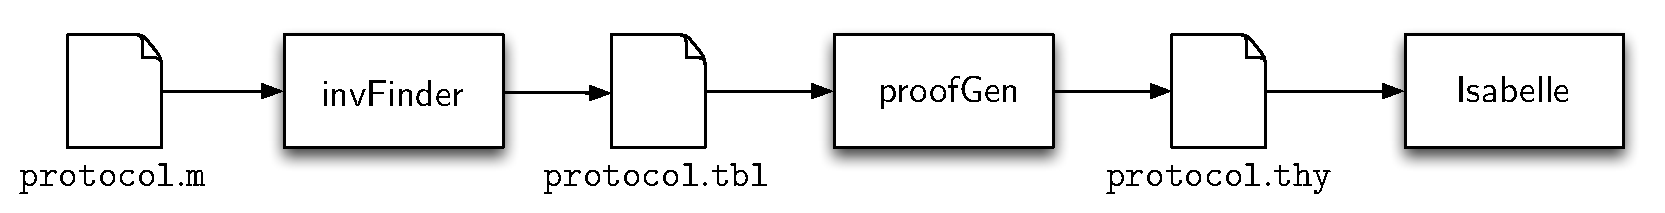
\includegraphics[width=1.0\textwidth]{paraVerifier.pdf}
%\vspace{-2cm}
 \caption{The general architecture of our parameterized
verification}
\label{fig:arch}
\end{figure}
 %\vspace{1cm}
%

%It is the task of {\sf paraVerifier} to construct each one of the
%remaining invariants by checking the causal relation between an
%invariant and a rule instance.


\section{The Searching Algorithm of the {\sf invFinder}}
The tool {\sf invFinder} works in a semi-proving and semi-searching
workflow. In an iterating step, it tries to prove some consistent
relation exists between an invariant and a rule, and automatically
generates a new auxiliary invariant if there is no such an invariant
in the current invariant set, and records the corresponding causal
relation information between the current rule and invariant. This
workflow is not finished until no new invariants is created.   The
core part of the searching algorithm of the {\sf invFinder} is given
roughly as follows,

\begin{specification}
1\twoSpaces let findInvsFromRule  chk choose  tautChk isNew rule inv newInvs invs casRel=\\
%2\twoSpaces  let rule=ruleApp pRule paras in\\
2\twoSpaces   val (g $\vartriangleright$ S)=rule in\\

3\twoSpaces   let inv'=preCond S inv in\\


4\twoSpaces   if  inv=inv' then\\

5\twoSpaces  \twoSpaces       let relItem=(rule,
inv,invHoldForRule2~inv~r) in\\
6\twoSpaces  \twoSpaces         (newInvs, relItem:casRel)\\


7\twoSpaces   else if  tautChk (g $\longrightarrow$inv') then\\
8\twoSpaces  \twoSpaces     let relItem=(rule, inv, invHoldForRule1~inv~r) in \\
9\twoSpaces  \twoSpaces        (newInvs, relItem:casRel)   \\


10\oneSpace   else let  candidates= subsets (decompose ((dualNeg inv') $\andc$ g ))  in\\

11\twoSpaces  \twoSpaces  let newinv =  choose chk candidates in\\
%12\twoSpaces       val ($\neg$ andList [items])=inv' in\\
%13\twoSpaces       let newinv= $\neg$ (andList ([items]@(and2Ands ant) )) in\\


12\twoSpaces  \twoSpaces     let relItem=(rule, inv,  invHoldForRule3 inv newInv   ) in\\

13\twoSpaces  \twoSpaces   if   ((isNew newInv (newInvs@invs)) then\\
14\twoSpaces  \twoSpaces   (newInvs@[normalize newInv], relItem\#casRel)\\
15\twoSpaces  \twoSpaces   else (newInvs,  relItem\#casRel)\\


16\oneSpace  else  error ``no new invariant";\\
\end{specification}


%{\sf invFinder} is implemented by FL, which is an excellent STE-tool
%of Intel \cite{}.
The tool {\sf invFinder} also depends on some oracle. {\tt
chk} is an oracle that checks whether a ground formula  is an
invariant in a given small reference model of the protocol. Such an
oracle can be implemented by firstly translating the formula in our modelling language into a
formula in SMV, and then calling  SMV to check whether it is an
invariant.  {\tt tautChk} is an oracle to check whether a formula is
a tautology, which is evaluated to be true at any state. Such a tautology checker for the formula $inv'$  is
implemented translating the formula into a form in SMT (abbrv for
SAT Modulo Theories) format, and then calls an SMT solver such as Z3
to check it.

  The above function {\sf findInvsFromRule} tries to find new
invariants and construct the causal relation between the rule
instance $rule$. %The statement {\tt
%cond => te|fe} is an abbreviation of the if-then-else expression
%that if $cond$ is true then $te$ else $fe$.
Parameters $newInvs$, $invs$, and $casRel$ are new invariants, invariants, and all the
causal relations constructed up to now, the above oracle functions
are also passed as parameters.  % Causal relations  are still not
%checked between the ones in $newInvs$ and rules.
The returned result
is updated new invariants,  and causal relations.
%

\begin{description}
\item[(1)] After computing the pre-condition {\tt inv'=preCond~S~inv} at line 3,
{\sf invFinder} performs case analysis on $inv'$: if {\tt inv=inv'},
 which means that no change made to $inv$ by statement $S$, then the new causal
relation item marked with tag {\tt invHoldForRule$_2$} is recorded
between $rule$ and $inv$, but at this moment there are no new
invariants to be added; for instance, let {\tt rule=crit 3},  {\tt inv=mutualInv~1~2}, thus
{\tt inv'=preCond~S~inv=inv}, then only a new relation item {\tt (crit 3, inv, invHoldForRule$_2$,\_)} will be added.

\item[(2)] Secondly, if {\tt tautChk g $\longrightarrow$inv'} is true, then
the new causal relation item marked with tag
{\tt invHoldForRule$_1$} is recorded between $rule$ and $inv$, but at this
moment there are no new invariants to be added either. For instance, let {\tt rule=crit~2}, {\tt inv=invOnX$_1$~1},
{\tt inv'=preCond~S~inv=$\neg_C$(false$\eqc$true $\andc$ n[1]$\eqc$C)}, obviously, {\tt
g $\longrightarrow_C$ inv'} holds forever because $inv'$ is always evaluated true,
 thus a new relation item {\tt (crit~2, inv, invHoldForRule$_1$,\_)} will be added.


 \item[(3)] Thirdly,  a new auxiliary invariant $newInv$ will be constructed, which will make the causal relation {\tt invHoldForRule$_3$} holds. Function {\tt dualNeg ($\neg_C$ f)} returns f; The function {\tt decompose f } decomposes a formula {\tt f} into a lists of sub-formluas $f_i(i \le N)$ such that each $f_i$ is not of a conjunction form and $f$ is semantically equivalent to $f_1 \andc ...\andc  f_i\andc  ...\andc f_N$. The function {\tt subsets fs} constructs all  subsets of fs, thus
    line 10  decomposes  ((dualNeg inv') $\andc$ g ) into a set of subformulas and constructs  candidates. The function {\tt choose} at line 12 chooses a proper  one from candidates, and construct a new invariant $newInv$. {\tt choose} need call {\tt chk} to
guarantee that the constructed formula is an invariant in the given
reference model; and function {\tt isNew} is used to check whether
the invariant is new. If yes, the invariant will be normalized, then be  added into $newInvs$,
 and the new causal relation item marked with tag {\tt invHoldForRule$_3$} will be added into the causal relations.
Here, the meaning of the word ``new" is modulo to the symmetry
relation. For instance, $\mathsf{mutualInv}~1~2$ is equivalent to
$\mathsf{mutualInv}~2~1$ in a symmetry view. The {\tt normalize} function normalizes the numbering order of the use of parameters in the invariant $inv$.
The result formula should be   a normal form, whose parameters
  always start from 1, and increase one by one if there are more
  parameters. Namely,  $\neg_C (x\eqc\mathsf{true} \andc n[1]\eqc\mathsf{C})$ is normalized, but
  $\neg_C$ (x$\eqc\mathsf{true} \andc n[2]\eqc\mathsf{C}$  not.    Let {\tt invs=newInvs=$\emptyset$}, {\tt rule=crit~1}, {\tt inv=mutualInv~1~2},
{\tt inv'=$ \mathsf{preCond}$~S~inv=$\neg_C$(true$\eqc$true $\andc$ n[2]$\eqc$C)}, from all the subsets of {\tt\{n[1]$\eqc$T, x$\eqc$true, n[2]$\eqc$C\}}, the {\tt choose} oracle selects the subset {\tt\{ x=true, n[2]$\eqc$C\}} combines all the item in this candidate, then constructs a new invariant {\tt $\neg$(x$\eqc$true $\andc$
   n[2]=$\eqc$C)}. After   normalization, the new invariant {\tt $\neg$(x=true $\wedge$
   n[1]$\eqc$C)} will be added, and  a new relation item {\tt (crit~1, inv, invHoldForRule3, newInv)} will be added.


\end{description}


 The output of the {\sf invFinder}, which is stored in file {\tt mutual.tbl},  is shown in Table
\ref{label-ground-causal relation}. In the table,  each line records the    index of a normalized   invariant, name of a parameterized rule, the rule
  parameters to instantiate the rule, a causal relation between
  the ground invariant and a kind of causal relation which involves the kind and proper formulas
  $f'$   in need (which are used to construct
      causal relations $\mathsf{invHoldForRule}_3$). The auxiliary invariants found by {\sf invFinder} includes: $\mathsf{inv_2}  \equiv  \negc (\mathsf{x} \eqc true  \andc  n[1]=C)$, $\mathsf{inv_3}    \equiv \negc  ( n[1]=C \andc n[2]=E)$,
$\mathsf{inv_4}  \equiv  \negc (x \eqc \mathsf{true}  \andc  n[1]\eqc \mathsf{E})$,   $\mathsf{inv_5}    \equiv \negc  ( n[1]\eqc \mathsf{C} \andc n[2] \eqc \mathsf{C})$.

 \begin{table}[!t]
\centering \caption{A fragment of output of {\sf invFinder}}\label{label-ground-causal relation} % {\tt
%simpMutual.tbl}
\begin{tabular}{|c|c|c|c|c|  }
\hline
  rule& ruleParas&inv&causal relation &   f'  \\
\hline
  .. & ..&.. &..&.. \\

\hline
  crit  & [1]&inv$_1$ 1 2& invHoldForRule3 &inv$_2$~2 \\
\hline
  crit &[2]& inv$_1$ 1 2& invHoldForRule3 &inv$_2$~1  \\
\hline
  crit & [3]& inv$_1$ 1 2 & invHoldForRule2  & \\
\hline
  .. & ..&.. &..&.. \\
\hline
\hline
  crit  & [1]&inv$_1$ 1 & invHoldForRule3 &inv$_2$~2 \\
\hline
  crit &[2]& inv$_1$ 1 & invHoldForRule3 &inv$_2$~1  \\
\end{tabular}
\end{table}
%The main body of {\sf paraVerifier}'s algorithm iteratively calls
%the function {\sf findInvsFromRule}  by instantiating each
%parameterized rule with different actual parameters of the finite
%reference protocol model. This procedure is finished until no more
%5new invariants can be created.



For a parameterized rule {\tt pRule}, for an invariant formula $inv$
in $newInvs$, we need a policy to create a list of parameters�� each of which will be  used to
instantiate {\tt pRule} into an actual rule {\tt rule}, then call
{\tt findInvsFromRule} to  check causal relations and find new
invariants. How many instantiations are needed? Here the underlying
instantiation principle should guarantee that each typical proof
case in parameterized causal relation analysis, which will be used
in parameterized proofs, should be covered by a ground causal
relation. The samples are enough to cover the proof pattern used in
parameterized  proofs. That is to say, if we regard the finite
instantiations as samplings, we must guarantee that
 the samples are enough to   be generalized in {\sf proofGen}
to parameterized forms  to finish  parameterized proofs.

In order to explain our parameter instantiation policy, we need introduce the concept of semi-permutation (or permutation moduolto symmetry) $\mathsf{SemiP}_{m}^{n}$. %Intuitively, we choose $n$ elemnts from %$[1,2...,m](n\le m)$  and put them in $n$ positions, when the choosed element is greater than $m-n$, we %need not consider its position, otherwise, we need consider its position.
Intuitively, a  semi-permutation is a permutation, but two  semi-permutation $L$ and $L'$ is equivalent if and only if length of $L$ and $L'$ are the same, and  $L_i$ and   $L_i'$ are the same if $L_i \le m - n$.  Formally, we define a
 $L \sim_m^n L' \equiv (\mathsf{length} ~L =\mathsf{length}~ L') \wedge (\forall i. i<\mathsf{length} ~ L \wedge L_i \le m-n \longrightarrow L_i=L'_i)$.  For instance, m=5, n=2, $[1,2]\not\sim_5^2[2,1]$, and  $[3,4]\sim_5^2 [4,3]$. $[[L]]_{m}^{n}=\{L'. L' \in P_{m}^{n} \wedge L'\sim_m^nL\} $, $\mathsf{SemiP}_{m}^{n}=\{[[L]]_{m}^{n}. L \in P_{m}^{n} \}$.


 Suppose $\mathsf{paraNumOfInv}~inv=nI$, and $\mathsf{paraNumOfRule}~pr=nR$,  our policy
 is to compute the set  $\mathsf{SemiP}_{nI+nR}^{nR}$, one representative of each element will be used as a group of parameters
 to instantiate $pr$. %For instance, $\mathsf{paraNumOfInv}~inv_1=2$, and $\mathsf{paraNumOfRule}~\mathsf{crit}=1$, then
  % [1],[2], and [3] will be used to instantiate $pr$ , this is corresponding to case (2) in the above discussion. For another instance, % $\mathsf{paraNumOfInv}~inv=2$, and $\mathsf{paraNumOfRule}~pr=2$, [1,2],[1,3],[1,4],[2,1],[2,3],[2,4],[3,1],[3,2],[3,4],[4,1], and [4,2] will be used to % instantiate $pr$.  notice that there is no [4,3] because it is symmetric to [3,4].
%
For a group parameters $L$, let $L_i=j$,  if $j \le nI$, then this parameter instantiation represents a parameterized case where  the $i-$th parameter of $pr$ is the same as the $j-$th element of parameters of $pInv$; otherwise  a parameterized case where  the $i-$th parameter of $pr$ is different from any  parameter of $pInv$.    Here we list two cases in {\sf mutual} to explain :
   \begin{itemize}
   \item When $\mathsf{paraNumOfInv}~pinv=1$ and $\mathsf{paraNumOfRule}~pRule=1$, for instance, $\mathsf{crit}$ and $\mathsf{inv}_3$ in Table \ref{label-ground-causal relation} are such a parameterized rule and invariant, $\mathsf{inv}_3~1$ is a normalized invariant,  then $\mathsf{SemiP}_{2}^{1}=[[1],[2]]$, we will use [1] and [2] to instantiate $\mathsf{crit}$  respectively. The sampling case $pInv~1$ and $pRule~ 1$ in the reference instance represents a parameterized case
    $pInv~\iInv_1$ and $pRule~ iR_1$ where $iR_1=\iInv_1$ in the parameterized instance, notice that $[1]!1=1$ ; the sampling case
    $pInv~1$ and $pRule~ 2$ in the reference instance represents a parameterized case $pInv~\iInv_1$
    and $pRule~ iR_1$ where $ iR_1\ne \iInv_1 $ in the parameterized instance, notice that  $[2]!1\ne 1$. Thus we   need instantiate $pRule$ with 1 and 2 respectively to obtain some $rule$ to find new invariants.

   \item When $\mathsf{paraNumOfInv}~pinv=1$ and $\mathsf{paraNumOfRule}~pRule=2$, for instance, $\mathsf{crit}$ and $\mathsf{inv}_1$ in Table \ref{label-ground-causal relation} are such a parameterized rule and invariant, $\mathsf{inv}_1~1~2$ is a normalized invariant, $\mathsf{SemiP}_{3}^{1}=[[1],[2],[3]]$,  we will use [1] and [2] and [3] to instantiate $\mathsf{crit}$ respectively.
     the sampling case $pInv~1~2$ and $pRule~ 1$ in the reference instance represents a
     parameterized case $pInv~\iInv_1~\iInv_2$ and $pRule~ iR_1$ where $iR_1=\iInv_1$ and $ iR_1 \ne \iInv_2$ in the parameterized instance, notice that $[1]!1=1$ and $[1]!1 \ne 2$ ;
     the sampling case $pInv~1~2$ and $pRule~ 2$ in the reference instance represents a parameterized
     case $pInv~\iInv_1~\iInv_2$ and $pRule~ iR$ where $iR_1=\iInv_2$ and $ iR_1 \ne \iInv_1$  in the parameterized instance, notice that $[2]!1=1$ and $[2]!1 \ne 2$ ;  the sampling case $pInv~1~2$ and
      $pRule~ 3$ in the reference instance represents a parameterized case $pInv~\iInv_1~\iInv_2$ and $pRule~ iR_1$
      where neither $\iInv_1=iR_1$ nor $\iInv_2=iR_1$ in the parameterized instance. Here we   need instantiate $prule$ with 1 and 2 and 3 respectively to obtain some $rule$ to find new invariants.
    \end{itemize}
%In order to  explain the idea of  finite sampling, we need recall our proof in Example \ref{caseSimp}. The typical proof pattern is based on case analysis  by %comparing the rule parameters such as $iR$ and invariant parameters such as $i_1$ and $i_2$. We also recall that the invariants searched by {\tt invFinder} are %always in a normal form, whose parameters
%  always start from 1, and increase one by one if there are more
 % parameters. The last, but not the least, is the symmetry of the cache coherence we exploit. Namely, a sampling case is one representative of an equivalence class  modulo to some symmetry relation.
The above  only informally explains the correspondence between concrete case and the accordingly  parameterized case by two instances, and we will formally define the correspondence which helps us to generalize the concrete cases searched by the {\sf invFinder} into parameterized cases which will be used in Isabelle proof.

%\section{Generalization}

\section{Generalization}
Intuitively, generalization means that a concrete index (formula or rule) is a representation of set of concrete indice (formulas or rules), which can be formalized  by a symbolic index (formula or rules) with side conditions specified by the constraint formulas. These constraint formulas can be formalized in our modelling languages in turn.    In order to formally define the parameterized model, we need extend our modelling language:

\begin{specification}
datatype indexType = scalar nat | formal string \\

datatype varType=Ident  string | Para varType indexType | Field  varType string\\

datatype valueType=enum string string |index indexType | boolV bool | symb string\\

%type\_synonym paramDefType= paramDef indexType valueType\\
%type\_synonym forallForm::paramDefType list $\Rightarrow$  formula  \\



%fun exitsForm::paramDefType list $\Rightarrow$ formula \\



\end{specification}

The most important extension is to adopt a symbolic (or formal) index, namely we can use
{\tt formal ``i1"} to formally a symbolic index $i_1$. The transformation from a scalar index to a symbolic index is straightforward: $\mathsf{indexTrans}~str~(\mathsf{scalar}~i) \equiv \mathsf{formal}~(str(\mathsf{nat2str}~i))$. With this transformation, we can lift some index transformation policy to value ( $\mathsf{indexTransval}$), var ( $\mathsf{indexTransvar}$), expression ($\mathsf{indexTransExp}$), formula ($\mathsf{indexTransForm}$), statement $\mathsf{indexTransStatement}$)and rule $\mathsf{indexTransRule}$).

\begin{specification}
letrec indexTransVar indTranspolicy (Ident str)= Ident str \\
\twoSpaces \alt indexTransVar indTranspolicy (Para v i)=Para (indexTransVar indTranspolicy i) (indTranspolicy i)\\
\twoSpaces \alt  indexTransVar indTranspolicy (Field v str)=Field (indexTransVar~indTranspolicy v) str\\

letrec indexTransval indTranspolicy (enum strt strv)= enum strt strv\\
\twoSpaces \alt indexTransval indTranspolicy (index ind)=index (indexTranspolicy i)\\
\twoSpaces \alt  indexTransval indTranspolicy (boolV b)=boolV b\\


letrec indexTransExp indTranspolicy (Ivar v)= Ivar (indexTransVar indTranspolicy  v)\\
\twoSpaces \alt indexTransExp indTranspolicy (Const v)=Const(indexTransval indTranspolicy v)\\
\twoSpaces \alt  indexTransExp indTranspolicy (f ? e1 :e2 )=\\
\twoSpaces \alt (indexTransForm indTranspolicy f) ? (indexTransExp indTranspolicy e1):indexTransExp indTranspolicy e2)\\
and
letrec indexTransForm indTranspolicy (eqn e1 e2)= eqn (indexTransExp indTranspolicy e1) (indexTransExp indTranspolicy e2)\\
\twoSpaces \alt indexTransForm indTranspolicy (neg f)=neg (indexTransForm indTranspolicy f)\\
\twoSpaces \alt  indexTransForm indTranspolicy (andForm f1 f2)=andForm (indexTransForm indTranspolicy f1) (indexTransForm indTranspolicy f2)\\
%\twoSpaces (indexTransForm indTranspolicy f) ? (indexTransExp indTranspolicy e1):indexTransExp indTranspolicy e2)\\
%let diffConGen len e=map ($\lambda$ L. mutualDiff e L$!1$ L$!2$) (comb len 2)\\
%let exNP~N~NP~str~P =
%\twoSpaces  let paramDefL=map ($\lambda$ i. (para$_i$,N)) (1 upto NP) in\\
%\twoSpaces    exitsForm ~paramDefL~ (diffConGen ~NP ~para) $\wedge_C$~ P)\\
\end{specification}


We write {\tt str$_j$} for {\tt $\mathsf{Const}~(\mathsf{index}~ \mathsf{indexTrans}~str~i)$} in the remaining parts of this work, where {\tt str} is a string:

%Now we formally define the generalization from a concrete case to a parameterized case:

If a formula (rule) contains an index $i$, then an implicit constraint is the index should be less than $N$ in a $N-$parameterized model. %This implicit constraint will play a role in the generation of
%actual formulas( rules) of $N-$parameterized model in Isabelle syntax.
Besides, if a formula such as {\tt mutualEx} contains more than one index, we require that indices should be mutually different. In order to  define the mutual difference between parameters of an invariant (or a rule), we need a function $\mathsf{comb}~m~n$ to compute a combination of $n$ elements from $n$ elements: $C_m^{n}$. For instance, $C_3^{2}=[[1,2],[1,3],[2,3]]$.

\begin{specification}
let mutualDiff str i j= $\neg_C$(  str$_i=_C$ $str_j)$ \\
%\twoSpaces
let diffConGen len str=map ($\lambda$ L. mutualDiff str L$!1$ L$!2$) (comb len 2)\\
%let exNP~N~NP~str~P =
%\twoSpaces  let paramDefL=map ($\lambda$ i. (para$_i$,N)) (1 upto NP) in\\
%\twoSpaces    exitsForm ~paramDefL~ (diffConGen ~NP ~para) $\wedge_C$~ P)\\
\end{specification}

% where $para$ is a string, and $P$ is a formula on the indice $para_i(0<i\le NP)$.

For instance, $\mathsf{diffConGen} ~3 ~str=[\neg_C(str_1=_C str_2),\neg_C(str_1=_C str_3),\neg_C(str_2=_C str_3)]$

% $\mathsf{diffConGen} ~3 ~i=[\neg_C(\mathsf{Const}~ (\mathsf{index}~i_1))=_C(\mathsf{Const}~ (\mathsf{index}~i_2))$, $\neg_C(\mathsf{Const}~ %(\mathsf{index}~i_1))=_C(\mathsf{Const}~ (\mathsf{index}~i_3))$,$\neg_C(\mathsf{Const}~ (\mathsf{index}~i_2))=_C(\mathsf{Const}~ (\mathsf{index}~i_3))$]. Intuitively, a %concrete formula like $\mathsf{mutual}~1~2$ will be generalized to a symbolic formula  $\mathsf{mutual}~i_1~i_2$ with side constraint $\neg_C(\mathsf{Const}~ %(\mathsf{index}~i_1))=_C(\mathsf{Const}~ (\mathsf{index}~i_2))$.


In order to formalize case analysis on the parameters of a rule and an invariant, which is generalized from a line in a causal table discussed in section \ref{},  we introduce the following definitions.

\begin{specification}
let neqL k L =
\twoSpaces  map ($\lambda$ j. $\neg_C$ ( iR$_k$ $=_C$ \iInv$_j$))   L\\

let indexCondGen nI  j k=\\
\twoSpaces  if (j $\le$ nI) then   (\iR$_k$$=_C$\iInv$_j$)\\ %\# (map neqL ((1 upto nI) subtract j) i))\\
\twoSpaces  else   (map neqL k  (1 upto nI) )\\


let caseGen lenInv rparas=map ($\lambda$ i. indexCondGen lenInv iInv iR (rparas ! $i$) ) (1 upto (length rparas))\\

let lookup lenInv   rparas i=if i$\le$lenInv then iInv$\_{i}$ else iR$_{find\_first~ (\lambda j. i=j) rparas }$\\
\end{specification}

where {\tt \iInv, \iR} are string ``\iInv", ``\iR" respectively.

Given a list of paramters {\tt rparas} to instantiate a rule, {\tt caseGen lenInv rparas} returns the assumptions on the case analysis of the rule parameters and invariant parameters, for instance,  {\tt caseGen 2 [1]=[[iR$_1$$=_C$\iInv$_1$] ]}; {\tt caseGen 2 [1,3]=[[iR$_1$$=_C$\iInv$_1$], [$\neg_C$iR$_2$$=_C$\iInv$_1$,$\neg_C$iR$_2$$=_C$\iInv$_2$]]}. {\tt find\_first~ ($\lambda$ j. i=j) rparas} returns the index of the first element which is equal to $i$.   {\tt lookup} is another parameter symbolic transformation policy to generalize a concrete index {\tt i}: if {\tt $\le$lenInv}, then {\tt i} will be transformed into  \iInv$\_{i}$, else return iR$\_{j}$ where $j$ is the index of $i$ in the list {\tt rparas}.

Now we formally define the generalization from a concrete case to a parameterized case, there are three generalization principles:
 \begin{description}
 \item[(1)] For a normalized concrete invariant formula  $cinv$ computed by {\sf invFinder}, $\mathsf{proofGen}$   generates a  record  {\tt symbForm \{name::string\} \{formFld::formula\} \{paraNumFld::nat\}  \{gFormFld::formula\}}, where field  {\tt name}  stores a string for the name of this invariant, formFld  symbolic formula $pInv=\mathsf{indexTrans2Form}~"\iInv"~$, paraNumFld the number of formal parameters of this invariant $NP=\mathsf{paraNumOfInv}~pInv$, and gFormFld a formula {\tt  diffConGen~NP~i} to specify a
     side constraint on the parameters of this invariant with this generalization, %, each of which is symmetric to $cinv$ for a permutation.
     $\mathsf{proofGen}$ creates a table {\tt symbInvs} to store all information of the symbolic invariant formulas.
     %$\mathsf{diffConGen}~(\mathsf{paraMumsOfInv}~cinv)~"\iInv"$ to specify  the assumptions that mutual difference between the parameters of the symbolic invariant. Here we assume that the string %$"\iInv"$ does not occur in $cinv$. In fact, the set $\{\mathsf{diffConGen}~(\mathsf{paraMumsOfInv}~cinv~"\iInv". $


 \item[(2)] $\mathsf{proofGen}$   generates  a  record  {\tt symbRule \{name::string\} \{ruleFld::rule\} \{paraNumFld::nat\}  \{gFormFld::rule\}} to store information on a symbolic rule, where field  {\tt name}  stores a string for the name of this rule, ruleFld  stores a  symbolic rule $prule$, which is translated from a rule in syntax in section \ref{sec:protocolSyntax}, and  paraNumFld the number of formal parameters of this symbolic rule $NP=\mathsf{paraNumOfRule}~pRule$,  and gFormFld a formula {\tt  diffConGen~NP~iR} to specify a
     side constraint on the parameters of this invariant with this generalization.  $\mathsf{proofGen}$ creates a table {\tt symbRules} to store all information of the symbolic invariant rules.%

     %a formula $\mathsf{diffConGen}~(\mathsf{paraMumsOfInv}~cr~"iR"$ to specify with the assumptions that mutual difference between the parameters of the symbolic invariant.  Here we assume that the string $"iR"$ does not occur in $cr$.

 \item[(3)]For an item {\tt (r,cinv,rparas,g,holdtype,f')} in a line of a causal table, suppose $cr=pr ~rparas$, $\mathsf{proofGen}$ generates  a  record  {\tt symbLine \{ruleName::string\} \{invName::string\} \{caseFld::formula\} \{branchFld::formula\} \{holdType::invHoldTagType\} \{hold3Form:formula option\}}. Here the filed caseFld is generated by $\mathsf{caseGen}~ lenInv~ rparas$   to specify the case condition between parameters of the invariant and rule, which is generalized from the causal line.  The field {\tt branchFld::formula} is  {\tt indexTransForm (lookup lenInv   rparas) g}, which speicies a case consition on some branch of some {\sf if} expression. The filed holdType is to indicate which causal relation are. If {\tt holdType=invHold3}, then {\tt hold3Form={\sf SOME} indexTransForm (lookup lenInv   rparas) f)}, else {\tt hold3Form={\sf NONE}}. $\mathsf{proofGen}$ creates a table {\tt symbCausalTab} to store all information of the symbolic causal relation.
 \end{description}
%-------------------------------------------------------------------------
\section{Automatical generation of Isabelle proof by {\tt proofGen}}
%-------------------------------------------------------------------------

A formal model in a theorem prover like Isabelle
includes the definitions of constants and rules and invariants,
lemmas, and proofs. An overview of the transformation strategy is
shown in Fig \ref{fig:mapping} from a protocol model in FL to
 the one in Isabelle.


 \begin{figure}[!ht]
% \centering %
 %\vspace{-0.8cm}
\includegraphics[width=1.0\textwidth]{isabelleScript.pdf}
%\vspace{-0.5cm}
 \caption{An overview of an Isabelle proof}
\label{fig:arch}
\end{figure}
% \vspace{1cm}
\subsubsection{Generating definitions of formal  rules and actual rules in a $N-$ parameterized model}
A formal definition of an invariant and all actual invariants of  $N-$parameterized model of $\mathsf{mutual}$ protocol is shown as follow:\\

\begin{specification}

 definition pinv4::nat $\Rightarrow$ formula   where [simp]:\\

       pinv4 \iInv1 $\equiv$\\

      neg ( andForm ( eqn ( IVar ( Global ''x'') )  ( Const true ))   \\

          ( eqn ( IVar ( Para ''n'' \iInv1) )  ( Const C )) )  \\

definition invariants::nat $\Rightarrow$ formula set  where [simp] :\\
invariants N$\equiv$ \{f. $\exists$ \iInv1 \iInv2. \iInv1 $\le$ N $\wedge$ \iInv2 $\le$ N $\wedge$ \iInv1 $\ne$ \iInv2 $\wedge$  f = pinv1 \iInv1 \iInv2  $\vee$ \\
 $\exists$ \iInv1. \iInv1 $\le$ N $\wedge$  f = pinv2 \iInv1   $\vee$\\
$\exists$ \iInv1 \iInv2. \iInv1 $\le$ N $\wedge$ \iInv2 $\le$ N $\wedge$ \iInv1 $\ne$ \iInv2 $\wedge$  f = pinv3 \iInv1 \iInv2  $\vee$\\
$\exists$ \iInv1. \iInv1 $\le$ N $\wedge$  f = pinv4 \iInv1  $\vee$\\
$\exists$ \iInv1 \iInv2. \iInv1 $\le$ N $\wedge$ \iInv2 $\le$ N $\wedge$ \iInv1 $\ne$ \iInv2 $\wedge$ f = pinv5 \iInv1 \iInv2  $\vee$   \}\\


\end{specification}

 For a record {\tt symbForm invName f num  sideConstraint} in the invariant table $symbInvTab$, the generation of its formal definition in Isabelle is rather straight-forward: {\tt invName} is used to the name of this invariant  this definition such as {\tt pinv4}, {\tt num} is used to define the type of this invariant formula such as {\tt nat $\Rightarrow$ formula}, and  {\tt f} is used to define the body of definition in Isabelle.  Besides, we also need to define the set of all the actual formulas of invariants
 in the $N-$parameterized model by {\tt invariants N}, each element of which can be an invariant formula instance. Notice that the constraints(assumptions) in the case condition such as {\tt $\exists$ \iInv1 \iInv2. \iInv1 $\le$ N $\wedge$ \iInv2 $\le$ N $\wedge$ \iInv1 $\ne$ \iInv2 $\wedge$  f = pinv1 \iInv1 \iInv2 } comes from two parts:  (1) the facts that all parameters of this invariant should be less than the parameter $N$; (2) the constraints from  {\tt sideConstraint}, which specifies that the mutual difference between two parameters.

\begin{specification}
letrec strsCat sepStr []=""\\
\alt strsCat sepStr [str]=str\\
\alt strsCat sepStr (str\#strs)=str \cat sepStr \cat  (strsCat sepStr strs)\\
 %strLs =itlist ($\lambda$ str1.$\lambda$ str2.str1 \cat sepStr \cat str2) strLs ""
let asmLess str SN i=str$_i$ \cat "$\le$ " \cat SN\\
%let asmsGen str sN len=itlist (\lambda i.\lambda str2.str2 \cat "" \cat (asmLess str SN i)) (map (\lambda i. str_i) (1 upto len)) " "\\
let asmsLookUp tab name fieldName=map form2Isabelle (fieldName (tbl\_element tab name))\\
let constraintGen symbInvs invName =\\
\twoSpaces   let asmsLessOnInv=asmsGen \iInv sN lenPInv in\\
\twoSpaces  let asmsMutualDiffOnInv=asmsLookUp symbInvs invName gFldName in\\
\twoSpaces strsCat "$\wedge$"  (asmsLessOnInv@asmsMutualDiffOnInv)   \\

let parasGen temp len =
  strsCat " " (map (index2Isabelle temp) ( 1 upto len)\\

let invParasGen lenPInv=parasGen \iInv lenPInv  \\

let frmDisj symbInvs invName=\\
\twoSpaces let constraint=constraintGen symbInvs invName in\\
\twoSpaces val (symbInv invN f  lenPInv gf)=tbl\_element symbInvs invName in\\
\twoSpaces let parasStr=invParasGen lenPInv in\\
\twoSpaces sprintf "$\exists$ \%s. \%s $\wedge$ f=\%s \%s" parasStr constraint invName parasStr\\

let frmsDisjs symbInvs  =\\
\twoSpaces strCat "$\vee$" (tbl\_map frmDisj symbInvs)\\

let actualInvsDefGen symbInvs=\\
\twoSpaces sprintf "definition invariants::nat $\Rightarrow$ formula set  where [simp] :\\
invariants N $\equiv$ \{f. \%s\}" (frmsDisjs symbInvs)\\
%let asmsMutualDiffOnInv=asmsLookUp symbInvs invName gFldName in
\end{specification}

In order to define the function to generate the definition all the actual invariants in the $N$-parameterized model, we define a function {\tt strsCat}, which concats a list of strings with a delimeter string {\tt sepStr}. {\tt asmLess} returns   a constraint that a parameter is less or equal to $N$. For instance, {\tt asmLess \iInv "N" 1="\iInv1$\le$N"}. {\tt parasGen} generates a string of parameters, which will applied to a name of a invariant formula (or a rule). For instance, {\tt parasGen \iInv 2="\iInv1 \iInv2"}. {\tt asmsLookUp} generates constraints of the mutual difference between two parameters, which can be looked up by the invariant name from the field  {\tt gFldName} storeded in a record;  {\tt frmDisj} generates a formula in Isabelle to specify a possible form of an invariant formula. For instance,  {\tt frmDisj symbInvs inv1="$\exists$ \iInv1 \iInv2. \iInv1 $\le$ N $\wedge$ \iInv2 $\le$ N $\wedge$ \iInv1 $\ne$ \iInv2 $\wedge$  f = pinv1 \iInv1 \iInv2"},\\  {\tt frmsDisjs} generates all the cases of the possible form of an invariant formula. With these predefined functions, {\tt actualInvsDefGen} generates the definition of all the invariant formulas: {\tt invariants N}.
%   For instance, let $gInv_4\equiv \neg (x=true \wedge n[1]=C)$, we define
%   a formal parameterized formula:
%  $pinv_4~i_1 \equiv
%  (x=true \wedge n[i_1]=C)$,
%  and $ex1P~N~(\lambda i.pInv~i)$ is all the actual formulas which are symmetric to $gInv$ in the N-parameterized
%  model of the protocol, and Spec \ref{} shows its Isabelle syntax of the invariant $pinv_4$ generated by {\tt proofGen}.
% {\tt  invariants N} is the set of all the actual rules. %;  for $gInv= (n[1]=C \wedge n[2]=C)$, we define an
%  $pInv~i_1~i_2=(n[i_1]=C \wedge n[i_2]=C)$, and $ex2P~N~(\lambda i~j.pInv~i~j)$ is all the formulas
%  which are symmetric to $gInv$ in the N-paramterized model of the
 % protocol. At last, we can define the set of all the auxiliary
 % invariants, which will be proved to be consistent with all the
 % rule.
% $ \mathsf{invariants} ~N \equiv \{f. ex1P~ N ~(\lambda i.  f= inv_{11}~ i)  ...\vee ex1P ~N ~(\lambda i.  f = inv_{1m}~ i )
%  \vee
% (ex2P~ N ~\lambda i ~j.  f= inv_{21}~ i~j)  ...\vee ex2P~ N ~(\lambda i~j.  f =inv_{2n}~ i~j
% ) \vee
%(ex3P~ N ~\lambda i ~j~k.  f= inv_{31}~ i~j~k)  ...\vee ex3P~ N
%~(\lambda i~j~k.  f =inv_{3o}~ i~j~k\}$, where $inv_{1i}$,
%$inv_{2j}$, and $inv_{3k}$ are formal invariant formulas with one,
%two three formal parameters respectively.  .


  Similar to the generation of   formulas, accordingly we can generate all the formal definition of rules and the actual rules used in the $N-$parameterized model by the table $symbRules$.

\subsubsection{Generating lemmas for causal relation between rules and invariants}
  Now we discuss how to use records on {\tt crit} and {\tt inv1} in the table $symbCausalTab$ to generate a lemma to prove causal relation hold between some rule $pr$ and some invarianr $inv_j$,
which will be applied in the proof of main lemma. An  example lemma
{\tt critVsinv$_1$} and its proof in Isabelle in the {\tt mutualEx} protocol, is illustrated as follows:


\begin{specification}
1lemma critVsinv1:\\
2  assumes  a1: $\exists$ iR1. iR1 $\le$ N $\wedge$ r=crit iR1 and \\
  a2: $\exists$  \iInv1 \iInv2. \iInv1 $\le$ N $\wedge$ \iInv2 $\le$ N $\wedge$ \iInv1 $\neq$ \iInv2 $\wedge$ f=inv1  \iInv1 \iInv2\\
3  shows  invHoldForRule f r (invariants
  N)\\
4  proof -\\
   from a1 obtain iR1 where a1:"iR1 $\le$ N $\wedge$ r=crit iR1" \\
   by blast\\
   from a2 obtain \iInv1 \iInv2 where \\
   a2:" \iInv1 $\le$ N $\wedge$ \iInv2 $\le$ N $\wedge$ \iInv1 $\neq$ \iInv2 $\wedge$ f=inv1  \iInv1 \iInv2"\\
   by blast \\
5  have iR1=\iInv1 $\vee$ iR1=\iInv2 $\vee$ (iR1 $\ne$ \iInv1 $\wedge$  iR1 $\ne$ \iInv2) by auto\\

6  moreover\{assume  b1:iR1=\iInv1\\
7  \twoSpaces have invHoldForRule3 (inv1 \iInv1 \iInv2) (crit iR1) (invariants N)\\
 \twoSpaces  \twoSpaces   proof(cut\_tac a1 a2 b1, simp, rule\_tac x=$\neg$ (x=true $\wedge$ n[\iInv2]=C)  in exI,auto)qed\\
8  \twoSpaces then have invHoldForRule f r
(invariants
  N)
by auto\}\\

9  moreover\{assume  b1:iR1=\iInv2\\
10 \twoSpaces have invHoldForRule3' (inv1 \iInv1 \iInv2) (crit iR1) (invariants N)\\
 \twoSpaces \twoSpaces   proof(cut\_tac a1 a2 b1, simp, rule\_tac x=$\neg$ (x=true $\wedge$ n[\iInv1]=C  in exI,auto)qed\\
11 \twoSpaces then have invHoldForRule f r (invariants
  N)
by auto\}\\

12   moreover\{assume  b1:(iR1 $\ne$  \iInv1 $\wedge$   iR1 $\ne$  \iInv2)\\
13 \twoSpaces have invHoldForRule2  f r  (invariants N)\\
  \twoSpaces \twoSpaces  proof(cut\_tac a1 a2 b1,  auto) qed\\
14 \twoSpaces then have invHoldForRule  f r
(invariants
  N)
by auto\} \\

15ultimately show invHoldForRule  f r
(invariants N)\\
16qed\\
\end{specification}

An lemma such as {\tt critVsinv1}  is generated by collecting all the records on the invariant {\tt inv1} and rule {\tt crit} in the table $symbRules$.
Line 2 are assumptions on the parameters of the invariant and rule, which come from four parts:  (1) the facts that all parameters of this invariant should be less than the parameter $N$; (2) the facts that all parameters of this invariant should be less than the parameter $N$; (3) the constraints of he mutual difference between parameters of the invariant (rule), which can be looked up in the field of those records  from the table $symbInvTab$ ($symbRuleTab$) by the invariant (rule) name {\tt inv1} ({\tt crit}), which specifies that the mutual difference between two parameters. line 5 splits cases of $iR1$ into all possible cases by comparing
$iR1$ with $\iInv_1$ and $\iInv_2$, which is the disjunction of all the {\tt caseFld} fields of these records. Lines 6-14  proves    these cases one by one: Lines 6-8 proves the case where {\tt iR1=\iInv1}; Lines 6-8 proves the case where {\tt iR1=\iInv2}; Lines 12-14 the case   where neither $iR1=\iInv_1$ nor $iR1=\iInv_2$.

%The aforementioned proof can be generated by instantiate the following pattern by replacing {\tt rule},
%{\tt inv}, {\tt proof1}, {\tt proof2}, {\tt proof3} with {\tt crit} and the detail proof lines 7-8, 11-12, and 14-15 respectively.
%This pattern works for each pair of a parameterized rule with two parameters and an invariant
%with two parameters.
%pattern of case analysis on the parameters  is determined by the number of parameters of
%the invariant and rule, which can be formalized by a proof template. Lines 1-5, 6, 9, 10, 13, 14, 17 18,19 can be resused by replacing the names of rule and
% invariant respectively.
%Detail proofs such as lines  7, 10, 13 are generated according to the lines on {\tt crit} and {\tt inv1} in Table \ref{}. The mapping is based on the symmetry mapping. Recall the  parameters instantiation policies we discussed in section \ref{},. {\t proof1} at line 7 is according with line in Table because the latter case is the representive of the former case in the sense of symmetry. These proofs are composed of two parts: a middle result to show which kind of causal relation should be choose to prove, then from this the conclusion can be obtained immediately.
%Thus  in  {\t proof1} should introduce a middle result $\mathsf{invHoldForRule_{3}}$, whose proof needs an existence construction by providing an auxiliary invariant formula {\tt $\neg$ (x=true $\wedge$ n[i2]=C}. {\t proof2} can be constructed similarly. {\t proof3} chooses $\mathsf{invHoldForRule_{2}}$ to prove,  , an {\tt auto} command is enough because such a goal can be solved automatically in Isabelle.




\begin{specification}
%letrec strsCat sepStr []=""\\
%\alt strsCat sepStr [str]=str\\
%\alt strsCat sepStr (str\#strs)=str \cat sepStr \cat  (strsCat sepStr strs)\\
 %strLs =itlist ($\lambda$ str1.$\lambda$ str2.str1 \cat sepStr \cat str2) strLs ""
%let asmLess str SN i=str$_i$ \cat "\dbRight<le> " \cat SN\\
%let asmsGen str sN len=itlist (\lambda i.\lambda str2.str2 \cat "" \cat (asmLess str SN i)) (map (\lambda i. str_i) (1 upto len)) " "\\
%let asmsLookUp tab name fieldName=map form2Isabelle (fieldName (tbl\_element tab name))\\
%let namedAsmTrans asmStr i="a" \cat (nat2str i) \cat ":" \cat asmStr\\
%let allNamedAsmsGen sN lenPInv lenPRule ruleName inVName symbRules symbInvs =\\
%\twoSpaces   let asmsLessOnInv=asmsGen \iInv sN lenPInv in\\
%\twoSpaces  let asmsLessOnRule=asmsGen iRule sN lenPRule in \\
%\twoSpaces  let asmsMutualDiffOnInv=asmsLookUp symbInvs invName gFldName in\\
%\twoSpaces  let asmsMutualDiffOnRule=asmsLookUp symbRules ruleName gFldName in\\
%\twoSpaces  let asmsOnInv=asmsLessOnInv@asmsMutualDiffOnInv in\\
%\twoSpaces  let asmsOnRule=asmsLessOnRule@asmsMutualDiffOnRule in\\
%\twoSpaces   let allAsms=asmsLessOnInv@asmsLessOnRule@asmsMutualDiffOnInv@asmsMutualDiffOnRule in\\
%\twoSpaces   let allNamedAsms=map ($\lambda$ (asmStr,i). namedAsmTrans asmStr i) (zip allAsms (1 upto (length %allAsms))) in\\
%\twoSpaces     strsCat " and " allNamedAsms\\




let rulePrarasGen lenPRule=parasGen iR lenPRule \\

let oneMoreBranch asmDepth asmForm proofStr=
\twoSpaces let asmName=asmDepth2Name asmDepth in
\twoSpaces sprintf\\
\twoSpaces "moreover\{assume  \%s:\%s\\
\twoSpaces \%s
\twoSpaces then have invHoldForRule (\%s i1 i2) (\%s iR) (invariants  N) \} by auto"\\
\twoSpaces (asmName, asmForm, proofStr, invName, ruleName)\\


let moreOversOnIfBra asmDepth causalLines =


let symbCausalRec2DisjItem asmDepth symbRec=\\
\twoSpaces  val (symbLine rnmae invName caseF holdTag formOpt)=symbRec in\\
\twoSpaces     form2Isabelle caseF\\

let symbCausalRecs2Allcases symbRecs=\\
\twoSpaces    strsCat "$\vee$" (map symbCausalRec2DisjItem symbRecs)\\

let proof3Gen caseF invHold3f=\\
%\twoSpaces sprintf\\
%\twoSpaces "moreover\{assume  b1:\%s\\
\twoSpaces have invHoldForRule3 f r (invariants N)\\
\twoSpaces  \twoSpaces   proof(simp, rule\_tac x=\%s  in exI,auto)qed\\
\twoSpaces \twoSpaces then have invHoldForRule f r
(invariants
  N)
\twoSpaces by auto"\\
%\twoSpaces (form2Isabelle caseF, \\
\twoSpaces (form2Isabelle invHold3f)\\


let symbCausalRec2Proof symbRec=\\
\twoSpaces  val (symbLine rnmae invName caseF caseG holdTag formOpt)=symbRec in\\
\twoSpaces     if (holdTag=invHold1) then \\
\twoSpaces      proof1Gen   caseF\\
\twoSpaces     else if  (holdTag=invHold2) then \\
\twoSpaces      proof2Gen   caseF\\
\twoSpaces     else proof3Gen   caseF invHold3f\\
\twoSpaces sprintf\\
\twoSpaces "moreover\{assume  b1:\%s\\
\twoSpaces then have invHoldForRule (\%s i1 i2) (\%s iR) (invariants  N) \} by auto"\\
\twoSpaces

let symbCausalRecs2Allproofs symbRecs=\\
\twoSpaces    strsCat " " (map symbCausalRec2Proof symbRecs)\\
\twoSpaces ultimately show invHoldForRule f r (invariants
  N) by auto\\

let lemmaOnCausalRuleInv ruleName invName symbRules symbInvs symCausalTab  =\\
\twoSpaces let allSymbRecs=filter ($\lambda$(symbLine rn invn caseF' holdTag' formOpt'). \\
\twoSpaces  (rn=ruleName) AND (invn=invName)) symCausalTab in\\
\twoSpaces let lenPInv=paraNumFld  (tbl\_element symbInvs  invName) in\\
\twoSpaces let lenPRule=paraNumFld  (tbl\_element symbRules  ruleName) in\\
\twoSpaces let asms1="a1:"  \cat (frmDisj symbInvs invName)   in\\
\twoSpaces let asms2="a2:"  \cat (ruleDisj symbInvs ruleName)   in\\
\twoSpaces let asms=asms1 \cat asms2 in\\
\twoSpaces let invParas=invParasGen lenPInv in\\
\twoSpaces let constraintOnInv= constraintGen symbInvs invName in\\
\twoSpaces let ruleParas=rulePrarasGen lenPRule in\\
\twoSpaces let constraintOnRule= constraintGen symbRules ruleName in\\
\twoSpaces let allDisjuncts=symbCausalRecs2Allcases allSymbRecs in\\
\twoSpaces let allSubProofs=symbCausalRecs2AllProofs allSymbRecs in\\
\twoSpaces sprintf\\

\twoSpaces"lemma \%sVs\%s:\\
%2  assumes  a2: iR $\le$ N and a3: i1 $\le$ N and a4: i2 $\le$ N\\ generations assumptions
\twoSpaces assumes \%s\\
\twoSpaces  shows  invHoldForRule (\%s \%s) (\%s \%s) (invariants
  N)\\
\twoSpaces  proof -\\
\twoSpaces from a1 obtain  \%s where a1:\%s $\wedge$ f=\%s \%s by auto\\
\twoSpaces from a2 obtain  \%s where a2:\%s $\wedge$ r=\%s \%s by auto\\
%5  have iR=i1 $\vee$ iR=i2 $\vee$ (iR $\ne$ i1 $\wedge$  iR $\ne$ i2) by auto\\ all cases
\twoSpaces5  have \%s  by auto\\
%6  moreover\{assume  b1:iR=i1\\
%7  \twoSpaces \%s\\
%8  \twoSpaces then have invHoldForRule (\%s i1 i2) (\%s iR)
%(invariants
%  N)
%by auto\}\\
%9  moreover\{assume  b1:iR=i2\\
%10  \twoSpaces \%s\\

%11 \twoSpaces then have invHoldForRule (\%s i1 i2) (\%s iR)
%(invariants
 % N)\\

%12   moreover\{assume  b1:(iR $\ne$  i1 ��   iR $\ne$  i2)\\
%13  \twoSpaces \%s\\
%14  \twoSpaces then have invHoldForRule (\%s i1 i2) (\%s iR)
%(invariants
 % N)  \\
\twoSpaces  \%s \\

\twoSpaces qed"\\

\twoSpaces (ruleName inVName,  \\
\twoSpaces asms, \\
\twoSpaces invParas,  constraintOnInv, invName, invParas, \\
\twoSpaces ruleParas,  constraintOnRule, ruleName, ruleParas, \\
\twoSpaces allDisjuncts, \\
\twoSpaces allSubProofs) \\
\end{specification}

{\tt namedAsmTrans asm i} adds a name "ai:" to a string of assumption in order to construct a named assumption. {\tt allNamedAsmsGen} generates all the aformentioned  four kinds of assumptions of the lemma in the previous paragrapgh: {\tt asmsLessOnInv} is according with (1) types of assumptions; {\tt asmsLessOnRule} (2) types of assumptions;  {\tt asmsMutualDiffOnInv} (3) types of assumptions; and {\tt asmsMutualDiffOnRule} (4) types of assumptions. After naming any one assumption with a name, {\tt allNamedAsmsGen} returns all the named assumptions which are conned by {\tt and} operator. {\tt symbCausalRec2Proof symbRec} generates a kind of proof in Isabelle according to a symbolic casual relation record {\tt symbRec}: if the tag of {\tt holdTag} is 1(2,3), then kind 1 (2,3) proof are generated accordingly. Here we list the most complex one: {\tt proof3Gen ruleName invName f}, which generates a proof which is according with {\tt invHoldType3} such as lines 6-8, and {\tt f} is another invariant formula which is needed to construct the {\tt invHoldType3} causal relation.  {\tt lemmaOnCausalRuleInv ruleName invName  symbRules symbInvs symCausalTab} returns a lemma on causal relation between  an invariant and a rule named {\tt  invName} and {\tt  ruleName} respectively: it first computes {\tt allSymbRecs } which are all symbolic causal relation records on {\tt  invName} and {\tt  ruleName},
 then  {\tt lenPInv} and {\tt lenPRule} which are numbers of the parameters of the invariant formula and rule, then {\tt asms} which are the assumptions part of the lemma such as line 2, {\tt allDisjuncts} the case analysis between the parameters of invariant and rule such as line 5, {\tt allSubProofs} all the proofs of the subcases such as lines 6-14, then fill all these into the blanks of the templates to generate the lemma.
%\twoSpaces  let asmsLessOnRule=asmsGen iRule sN lenPRule in \\
%\twoSpaces  let asmsMutualDiffOnInv=asmsLookUp symbInvs invName gFldName in\\
%\twoSpaces  let asmsMutualDiffOnRule
\subsubsection{Generating proofs for the main lemma}

%-------------------------------------------------------------------------
At last, we discuss how to create automatically the proof for the main lemma, which depends
 on the applying the lemmas which are created in subsection \ref{sec:genOfIsabelleProof}.  The consistency lemma is our
main weapon to prove, which requires proving two parts of
obligations.



\begin{description}
\item[(1)] For any invariant $inv \in (\mathsf{invariants} ~N) $,  any
state $s$, if $ini$ is evaluated true at state $s$, then $inv$ is
evaluated true at state $s$.
\item[(2)]  For any invariant $inv \in (\mathsf{invariants} ~N)$, any $r$ in rule set
$ \mathsf{rules} ~N$ , one of the causal relations
$\mathsf{invHoldForRule}_{1-3}$ holds.
\end{description}
%
%Proof of Part (1) is  simple. %%For an invariant
%$inv=\mathsf{implyForm}~ant~cons$ in $invs$, we only need to prove
%that either $ant$ is evaluated as false or $cons$ is evaluated true
%at an initial state $s$ in order to prove $\mathsf{formEval}
%~inv~s$. Such a proof  can be automatically solved by Isabelle's
%$\mathsf{auto}$ command.
An overview of a formal proof of Part (2) generated by {\tt
proofGen} is illustrated as follows. The proof of part (2) in the proof of the consistency theorem is based on the two levels of case analysis on the form of rules and the invariants.
 In the first level, we do case analysis on the form of rules, then we do case analysis on the form of invariants.
For a case on proving the existence of casual relation between {\tt ruleName} and {\tt invName}, we solve the subgoal by the lemma  {\tt ruleNameVsinvName} such as {\tt critVsInv1}.


\begin{specification}
lemma main:
  $\isasymlbrakk$  s$\in$ reachableSet \{ mutualIni  N\} (rules N); 0<N$\isasymrbrakk$\\
  $\Longrightarrow$ $\forall$ inv. inv $\in$ (invariants N) $\longrightarrow$ formEval inv s\\
proof(rule consistentLemma)\\
 % show consistent (invariants N) \{mutualIni  N\} (rules N)\\
 % proof(cut\_tac a1, unfold consistent\_def,rule conjI)\\
%~~    show  $\forall$inv ini s. inv $\in$ (invariants N)
%$\longrightarrow$ ini $\in$\{mutualIni  N\}$\longrightarrow$formEval
%ini s $\longrightarrow$ formEval inv s\\
%  ~~ proof((rule allI)+,(rule impI)+)\\
% ~~~~ ......\\
%   ~~~~   fix inv ini s\\
%  ~~~~    assume b1:inv $\in$ (invariants N) \\
%  ~~~~    and b2:ini $\in$
%{mutualIni  N}  and b3:formEval ini s\\
%    ~~~~  show formEval inv s\\
%   ~~~~   proof -\\
%
%   ~~~~~~     have c1:      exLessP N (\%i.  inv= inv1 i) $\vee$exLessP N (\%i.  inv= inv2 i) $\vee$
%    ex2P N (\%i j. inv=inv3 i
%   j) \\$\vee$ ex2P N (\%i j. inv=inv4 i j)$\vee$ex2P N (\%i j. inv=inv5 i j)\\%$\vee$\\
% %  ~~~~~~~~                     ex2P N (\%i j. inv=mutualInv3 i j)\\

%    ~~~~~~       by (cut\_tac b1, simp add:invariants\_def)\\

%     ~~~~~~    moreover\\
%    ~~~~~~    \{assume d1: exLessP N (\%i.  inv= inv1 i)\\
%      ~~~~~~     have formEval inv s\\
%       ~~~~~~~~      by (metis b2 b3 d1 iniImplyInv.verify)\}\\
      % ~~~~~~~~   \}\\
       ~~~~~~~~   ......\\
     % ~~~~~~   moreover\\
     % ~~~~~~   \{assume d1: ex2P N (\%i j.  inv=inv5 i j)\\
     %  ~~~~~~    have formEval inv s\\
     %   ~~~~~~~~     by (metis b2 b3 d1 invInterp5.iniImplyInv)\}\\
       % ~~~~~~ \}\\
    %   ~~~~~~   ultimately show formEval inv s\\
     %   ~~~~~~ ~~   by blast\\

%    ~~~~    qed\\

next   show  $\forall$inv r. inv $\in$ invariants N$\longrightarrow$
 r $\in$rules N$\longrightarrow$invHoldForRule inv r (invariants N) \\

   proof((rule allI)+,(rule impI)+)\\
\twoSpaces      fix f r \\
\twoSpaces         assume b1: f $\in$ invariants N  and b2:r $\in$ rules N\\

\twoSpaces      have c1: ($\exists$ iR1. iR1 $\le$ N $\wedge$ r=exit iR1)$\vee$\\
\twoSpaces  ($\exists$ iR1. iR1 $\le$ N $\wedge$ r=idle iR1)$\vee$ \\
\twoSpaces   ($\exists$ iR1. iR1 $\le$ N $\wedge$ r=crit iR1) $\vee$ \\
\twoSpaces  ($\exists$ iR1. iR1 $\le$ N $\wedge$ r=try iR1)\\
\twoSpaces\twoSpaces         by(cut$\_$tac  b2,auto)\\
\twoSpaces moreover\\
\twoSpaces\oneSpace $\{$assume c1: $\exists$ iR1. iR1 $\le$ N $\wedge$ r=exit iR1 \\

\twoSpaces\oneSpace have d1:   ($\exists$ \iInv1 \iInv2. \iInv1 $\le$ N $\wedge$ \iInv2 $\le$ N $\wedge$ \iInv1 $\ne$ \iInv2 $\wedge$  f = inv1 \iInv1 \iInv2)$\vee$ \\
\twoSpaces\oneSpace($\exists$ \iInv1.   \iInv1 $\le$ N $\wedge$    f = inv2 \iInv1 )$\vee$ \\
\twoSpaces\oneSpace ......\\
\twoSpaces\oneSpace ($\exists$ \iInv1 \iInv2. \iInv1 $\le$ N $\wedge$ \iInv2 $\le$ N $\wedge$ \iInv1 $\ne$ \iInv2 $\wedge$  f = inv5 \iInv1 \iInv2)  \\
\twoSpaces\twoSpaces   ~by (cut$\_$tac b1, simp )\\

\twoSpaces\oneSpace\twoSpaces  moreover\\
\twoSpaces\oneSpace\twoSpaces$\{$assume d1: $\exists$ \iInv1 \iInv2. \iInv1 $\le$ N $\wedge$ \iInv2 $\le$ N $\wedge$ \iInv1 $\ne$ \iInv2 $\wedge$  f = inv1 \iInv1 \iInv2\\


\twoSpaces\oneSpace \twoSpaces  have f r (invariants N) \\
\twoSpaces\twoSpaces\twoSpaces         by(cut$\_$tac  c1 d1, metis exitVsInv1)\}\\
\twoSpaces\twoSpaces\twoSpaces  ......\\
\twoSpaces\oneSpace\twoSpaces moreover\\
\twoSpaces\oneSpace\twoSpaces      $\{$assume d1: $\exists$ \iInv1 \iInv2. \iInv1 $\le$ N $\wedge$ \iInv2 $\le$ N $\wedge$ \iInv1 $\ne$ \iInv2 $\wedge$  f = inv5 \iInv1 \iInv2\\

\twoSpaces\oneSpace\twoSpaces ......~~~~          \\
\twoSpaces\oneSpace \twoSpaces  have invHoldForRule f r (invariants N) \\

\twoSpaces\twoSpaces\twoSpaces     by(cut$\_$tac c1 d1, simp) $\}$\\


\twoSpaces\oneSpace \twoSpaces ultimately have invHoldForRule f r (invariants N) \\

\twoSpaces\twoSpaces\twoSpaces     by blast \\%\}\\
\twoSpaces\twoSpaces\twoSpaces        $\}$\\

\twoSpaces  moreover\\
\twoSpaces\oneSpace  $\{$assume c1: $\exists$ iR1. iR1 $\le$ N $\wedge$ r=idle iR1\\

\twoSpaces\oneSpace \oneSpace  ......\\

\twoSpaces\oneSpace \oneSpace   \}\\
\twoSpaces ......\\
\twoSpaces                   ultimately show invHoldForRule f r (invariants N) ~~by blast\\
qed\\
qed\\


%next\\
%~~show s $\in$ reachableSet {mutualIni N} (rules N) ~~by (metis
%a1)\\
%
%next.... \\

%qed\\ %end\\
\end{specification}
%\vspace{-0.5cm}
 %in order to verify the cache coherence protocols. Others are straightforward.
The proof is a typically
readable one in Isar style \cite{}, which uses calculation
reasoning such as {\tt moreover} and {\tt ultimately} to do  case analysis on
the form of rules and the invariants. Lines 1-5 use proper Isabelle
proof commands to   decompose the main proof goal of forall  and
implication form,    fix a rule {\tt r} and {\tt inv}, then have two
assumptions {\tt  b1: inv$\in$ invariants N  and b2:r $\in$ rules
N}, now we need show the goal {\tt invHoldForRule f r (invariants
N)}. line 5 splits cases of $r$ into all possible cases according to
the definition of $rules~N$. %In order to save space, we adopt the following abbreaviation:
% $\mathsf{ex1P}~ N~ P \equiv \exists i. (i \le N \wedge P~
%i)$, $\mathsf{ex2P}~ N~ P \equiv \exists i~j. (i \le N \wedge j \le
%N \wedge i\ne j \wedge P~ i~j)$, and $\mathsf{ex3P}~ N~ P \equiv
%\exists i~j~k. (i \le N \wedge j \le N \wedge k \le N\wedge i\ne j
%\wedge i\ne k \wedge j\ne k \wedge P~ i~j~k)$.
Line 6 starts the case analysis on
$r=r_0$. Line 7 again splits cases of $inv$ into all possible cases
according to the definition of $invariants~N$. Line 8-10 proves the
goal at case when $r=exit$ and $inv=inv1$. At line 10,  a  proved
lemma {\tt exitVsInv1}  is directly applied to solve the proof
goal.  Similiarly, we can do subproofs on other cases on {\tt inv},
and finish the proof goal accordingly.
 After finishing the proof of the last case  of $inv=inv5$,
 we finish the proof of the first case $r=exit$. Similarly, we can
 finish the proof goal at
each subcase on {\tt r}. At  lines 19 and  20 we show we have
finished the proof goal formally.


\begin{specification}
let oneCaseOnInv symbInvs ruleName invName =\\
val (symbIn invN inv len gf)=tbl\_element symbInvs invName in\\
sprintf "
moreover\\
\twoSpaces\oneSpace\twoSpaces$\{$assume d1: \%s\\


\twoSpaces\oneSpace \twoSpaces  have f r (invariants N) \\
\twoSpaces\twoSpaces\twoSpaces         by(cut$\_$tac  c1 d1, metis \%sVs\%s)\}"\\
(frmDisj symbInvs invName,\\
 ruleName, invName);\\

let allCasesOnInvs symbInvs ruleName=\\
 let allInvns=tbl$\_$keys symbInvs in\\
 let allCasePfs=map (oneCaseOnInv symbInvs ruleName ) allInvn in\\
 strCat "$\backslash$n"  allCasePfs;\\

let oneCaseOnRule symbInvs symbRules ruleName =\\
let constraint=constraintGen symbRules ruleName in \\
val (symbRule rN r lenR gf)=tbl\_element symRules ruleName in\\
let parasStr=ruleParasGen lenR in\\
sprintf "\\
\twoSpaces moreover\\
\twoSpaces\oneSpace $\{$assume c1: \%s \\

\twoSpaces\oneSpace have d1:   \%s\\
\twoSpaces\twoSpaces   ~by (cut$\_$tac b1, simp )\\
\twoSpaces\twoSpaces \%s\\
\twoSpaces\oneSpace ultimately have invHoldForRule f r (invariants N) \\

\twoSpaces\twoSpaces\twoSpaces     by blast \\%\}\\
\twoSpaces\oneSpace        $\}$"\\
(ruleDisj symbRules ruleName,\\
 frmsDisjs symbInvs,   \\
 allCasesOnInvs ruleName symbInvs);\\
 \\

let allCasesOnRules symbInvs symbRules=\\
 let allRns=tbl$\_$keys symbRules in\\
 let allCasePfs=map (oneCaseOnRule symbInvs symbRules) allRns in\\
 strCat "$\backslash$ n"  allCasePfs;\\

let mainThmGen symbRules symbInvs=\\
sprintf\\
"theorem main:\\
  $\isasymlbrakk$  s$\in$ reachableSet \{ mutualIni  N\} (rules N); 0<N$\isasymrbrakk$\\
  $\Longrightarrow$ $\forall$ inv. inv $\in$ (invariants N) $\longrightarrow$ formEval inv s\\
proof(rule consistentLemma)\\
 % show consistent (invariants N) \{mutualIni  N\} (rules N)\\
 % proof(cut\_tac a1, unfold consistent\_def,rule conjI)\\
%~~    show  $\forall$inv ini s. inv $\in$ (invariants N)
%$\longrightarrow$ ini $\in$\{mutualIni  N\}$\longrightarrow$formEval
%ini s $\longrightarrow$ formEval inv s\\
%  ~~ proof((rule allI)+,(rule impI)+)\\
% ~~~~ ......\\
%   ~~~~   fix inv ini s\\
%  ~~~~    assume b1:inv $\in$ (invariants N) \\
%  ~~~~    and b2:ini $\in$
%{mutualIni  N}  and b3:formEval ini s\\
%    ~~~~  show formEval inv s\\
%   ~~~~   proof -\\
%
%   ~~~~~~     have c1:      exLessP N (\%i.  inv= inv1 i) $\vee$exLessP N (\%i.  inv= inv2 i) $\vee$
%    ex2P N (\%i j. inv=inv3 i
%   j) \\$\vee$ ex2P N (\%i j. inv=inv4 i j)$\vee$ex2P N (\%i j. inv=inv5 i j)\\%$\vee$\\
% %  ~~~~~~~~                     ex2P N (\%i j. inv=mutualInv3 i j)\\

%    ~~~~~~       by (cut\_tac b1, simp add:invariants\_def)\\

%     ~~~~~~    moreover\\
%    ~~~~~~    \{assume d1: exLessP N (\%i.  inv= inv1 i)\\
%      ~~~~~~     have formEval inv s\\
%       ~~~~~~~~      by (metis b2 b3 d1 iniImplyInv.verify)\}\\
      % ~~~~~~~~   \}\\
       ~~~~~~~~   ......\\
     % ~~~~~~   moreover\\
     % ~~~~~~   \{assume d1: ex2P N (\%i j.  inv=inv5 i j)\\
     %  ~~~~~~    have formEval inv s\\
     %   ~~~~~~~~     by (metis b2 b3 d1 invInterp5.iniImplyInv)\}\\
       % ~~~~~~ \}\\
    %   ~~~~~~   ultimately show formEval inv s\\
     %   ~~~~~~ ~~   by blast\\

%    ~~~~    qed\\

next   show  $\forall$inv r. inv $\in$ invariants N$\longrightarrow$
 r $\in$rules N$\longrightarrow$invHoldForRule inv r (invariants N) \\

   proof((rule allI)+,(rule impI)+)\\
\twoSpaces      fix f r \\
\twoSpaces         assume b1: f $\in$ invariants N  and b2:r $\in$ rules N\\

\twoSpaces       have c1:\%s\\

\twoSpaces\twoSpaces         by(cut$\_$tac  b2,auto)\\
\twoSpaces\twoSpaces\%s
\twoSpaces                   ultimately show invHoldForRule f r (invariants N) ~~by blast\\
qed\\
qed"\\

(rulesDisjs symInvs,
allCasesOnRules symbInvs symbRules)
%next\\
%~~show s $\in$ reachableSet {mutualIni N} (rules N) ~~by (metis
%a1)\\
%
%next.... \\

%qed\\ %end\\
\end{specification}

function {\tt oneCaseOnInv} generates  one proof for the existence of causal relation between an invariant named {\tt invName} and   a rule {\tt ruleName};  {\tt allCasesOnInvs symbInvs ruleName} generates  all the  proofs for the existence of causal relation between any invariant in {\tt symbInvs} and   a rule named {\tt ruleName}; {\tt oneCaseOnRule symbInvs symbRules ruleName} combine necessary

%=========================================
\section{Verification products}
%=========================================

After the auxiliary invariants are found,  the formula set $\mathsf{pinvs}~ N$ in Table \ref{} can be used to analyze
 and verify the design  of the protocol. In fact, they gives a complete
logical characterization of the semantics of the protocol. It will gives a deep insight of the protocol. These properties are divided into two categories: (1) correspondence between
control signals; (2)mutual exclusion between control signals. For instance, the intuitive meaning of the invariants is analyzed as follows:

\begin{table}[htbp] \label{Summarization of invariants}
\centering \caption{Summarization of invariants}
\begin{tabular}{|c|c| }
\hline
invariant &  meaning  \\
\hline
$\mathsf{invOnX_1} ~i$& Once some n[i] is set C, the flag x will be set false \\
\hline
$\mathsf{invOnX_2} ~i$&  Once some n[i] is set E, the flag x will be set false \\
\hline
$\mathsf{mutualInv}~ i ~j$ &  the mutual exclusion between n[i]=C and n[j]=C \\
\hline
$\mathsf{aux}_1~ i ~j$ &  the mutual exclusion between n[i]=C and n[j]=E \\
\hline
$\mathsf{aux}_2~ i ~j$ &  the mutual exclusion between n[i]=C and n[j]=E \\
\hline
\end{tabular}
\end{table}
%$\mathsf{invOnX_1} ~i$ specifies that the flag $x$ shows the
%availability of the critical section. Once some node state variable
%$n[i]$ is set $C$ or $E$, $x$ will be set $true$. Formulas
%$\mathsf{mutualInv}~ i ~j$, $\mathsf{aux_1} ~i~j$, and
%$\mathsf{aux_2} ~i~j$ state the mutual exclusion properties between
%a node's $\mathsf{C}(\mathsf{E})$ state and another different node's
%$\mathsf{C}(\mathsf{E})$ state.
The causal relations listed in Table \ref{} only illustrate why the invariants hold forever at each reachable state set.
That is to say, for a rule $r$ and an $inv$ descriibed in a line, one of the three causal relation $\mathsf{invHoldForRule}_{1\_3}$ holds, so an invariant holds after the execution the rule $r$. The Isabelle proof-script formally generalize these causal relation into parameterized form and proved the existence of the  causal relations. At last, a main lemma formally specifies that why the invariants hold forever at any reachable state set, and is formally proved by using the consistency lemma. In this sense, the Isabelle script can be seen as  a formal analysis document. The script contains 2243 line, and and costs more than 56
minutes for Isabelle to check in a 64-bit computing server platform which has a
160-multicore Intel Xeon CPU with 2.40GHz clock speed.


%=========================================
\section{Experiments}
%=========================================
We implement our tool in Forte \cite{Forte}. More experiments are
done including typical bus-snoopy ones such as MESI and MOESI,
 directory-based ones such as  Germanish, and  German protocols. The detail experiment codes and data can
be found in \JP{\cite{LiCache14}}. Each experiment data includes the
${\sf paraVerifier}$ model, invariant sets found, Isabelle proof
scripts, and the simulation flow graph of one single node. A table
summarizes  our experiments below. Among the benchmarks, the German
protocol   was posted
 as
% Among the benchmarks, a case study is done
%on a directory-based protocol, German protocol, which was posted as
a challenge to the formal verification community by Steven German in
2000. German protocol is a moderate case.
To the best of our knowledge, few people but us give a complete proof to verify
the mutual exclusion  property of the German protocol
 in a theorem prover.

 \begin{table}[htbp] \label{Summarization of experiment results}
\centering \caption{Summarization of results on benchmarks}
\begin{tabular}{|c|c|c|c|c|}
\hline
protocol &  ruleNum & invariantNum & time(s) & memory(M) \\
\hline
simpMutual& 4& 5 & 5.66 & 10.3 \\
\hline
MESI & 4& 3 & 4.66 & 11.5  \\
\hline
MOESI &  5& 3 &3.98 & 11.3  \\
\hline
 German-ish  & 6& 4 &35.8 & 15.1   \\
\hline
German & 13 & 48 & 1222.2 & 16.1   \\
\hline
\end{tabular}
\end{table}

%=========================================
\section{Conclusion}
%=========================================
Our case studies on cache coherence protocols are typical examples
to illustrate the guiding principle of {\sf paraVerifier}. The
 consistency lemma based on the induction approach, is the
core of our work, which gives the heuristics to guide the tool
 to search invariants. Instead of ``invisible invariants in previous work
 (see e.g,~\cite{Pnueli2001}, our invariants are visible,
 which can be further refined to precisely
 analyze the correctness of the protocol both in theoretical and practical aspects.

\bibliographystyle{splncsnat}
\bibliography{gste,cache,refer}
\end{document}
